%\documentclass{acmsiggraph}               % final
\documentclass[review]{acmsiggraph}      % review
%\documentclass[widereview]{acmsiggraph}  % wide-spaced review
%\documentclass[preprint]{acmsiggraph}    % preprint

%% Uncomment one of the four lines above depending on where your paper is
%% in the conference process. ``review'' and ``widereview'' are for review
%% submission, ``preprint'' is for pre-publication, and ``final'' is for
%% the version to be printed.

%% These two line bring in essential packages: ``mathptmx'' for Type 1 
%% typefaces, and ``graphicx'' for inclusion of EPS figures.

\usepackage{mathptmx}
\usepackage{graphicx}

%% use this for zero \parindent and non-zero \parskip, intelligently.

\usepackage{parskip}
\usepackage{subfigure}
\usepackage{smrdefaults}

%% If you are submitting a paper to the annual conference, please replace 
%% the value ``0'' below with your OnlineID. If you are not submitting this
%% paper to the annual conference, you may safely leave it at ``0'' -- it 
%% will not be included in the output.

\onlineid{papers\_0107}

%% need to document this!

\acmformat{print}

%% Paper title.

\title{TAPESTREA: Sound Scene Modeling By Example}

%% Author and Affiliation (single author).

\author{Ananya Misra, Perry R. Cook, and Ge Wang\\Princeton University\thanks{e-mail: \{amisra, prc, gewang\}@cs.princeton.edu}}

%% Author and Affiliation (multiple authors).

%%\author{Roy G. Biv\thanks{e-mail: roy.g.biv@aol.com}\\ Starbucks Research %
%%\and Ed Grimley\thanks{e-mail:ed.grimley@aol.com}\\ Grimley Widgets, Inc. %
%%\and Martha Stewart\thanks{e-mail:martha.stewart@marthastewart.com}\\ Martha Stewart Enterprises \\ Microsoft Research}

%% Keywords that describe your work.

%\keywords{sound scene, synthesis, sinusoidal modeling, wavelet}
% should sound texture be a keyword?

%%%%%% START OF THE PAPER %%%%%%

\begin{document}

\teaser{
\center
\includegraphics[width=6.5in]{teaser.eps}
%  \subfigure[original]{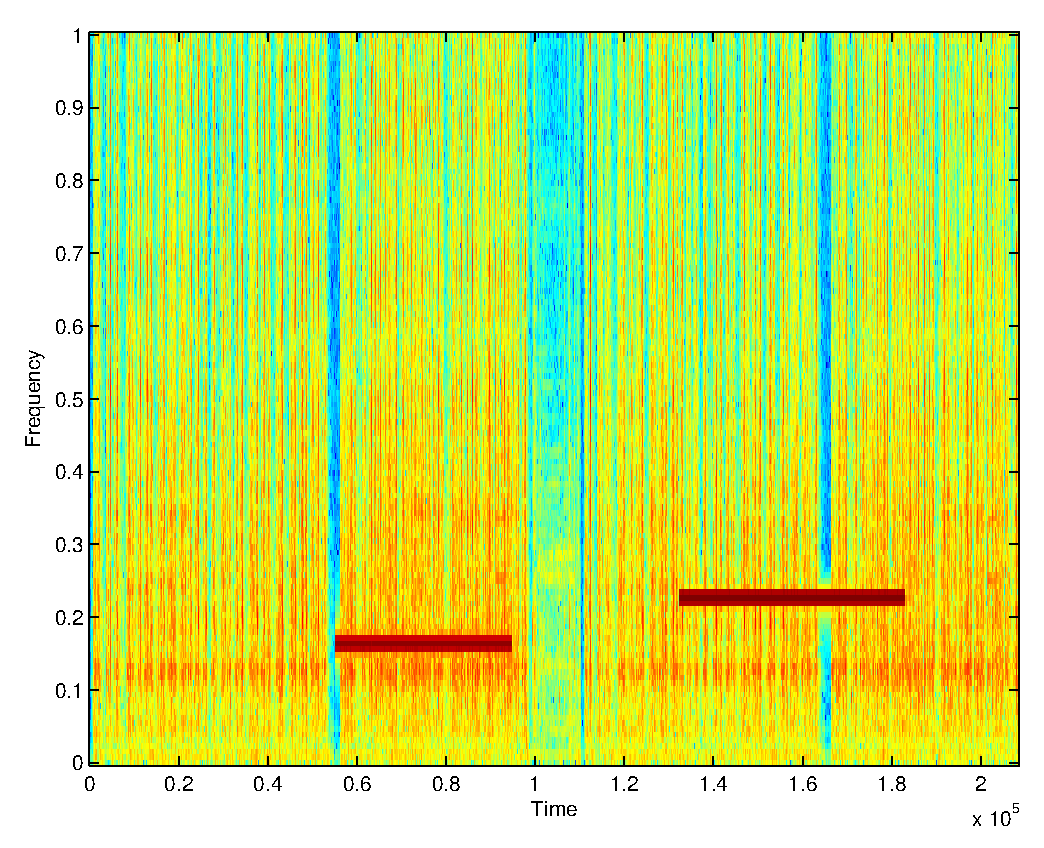
\includegraphics[width=.24\textwidth]{story1.eps}}
%  \subfigure[foreground]{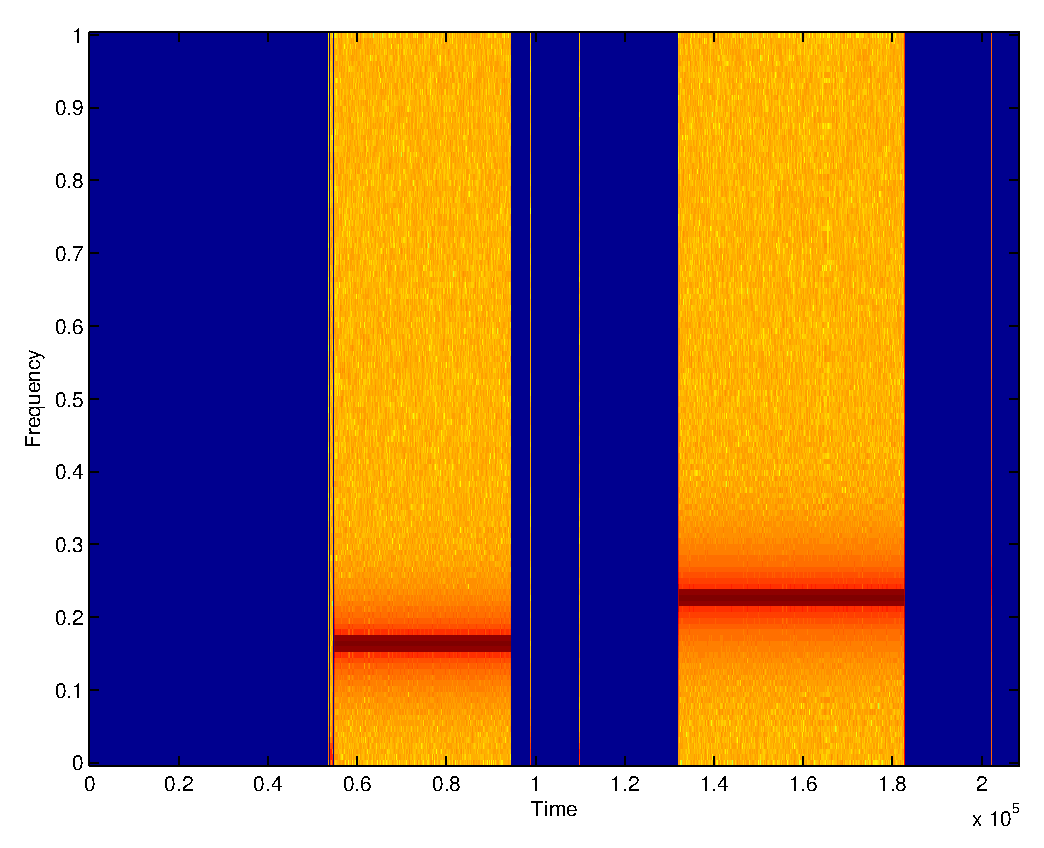
\includegraphics[width=.24\textwidth]{story2.eps}}
%  \subfigure[background]{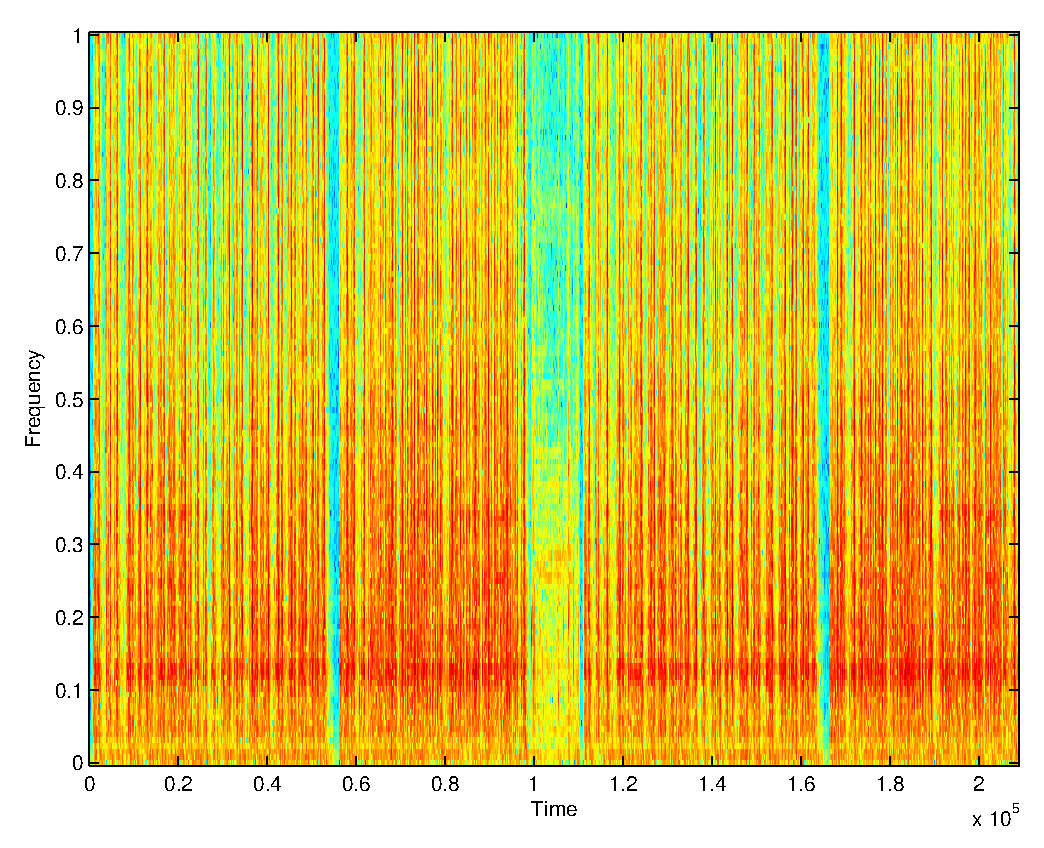
\includegraphics[width=.24\textwidth]{story3_fake.eps}}
%  \subfigure[synthesized]{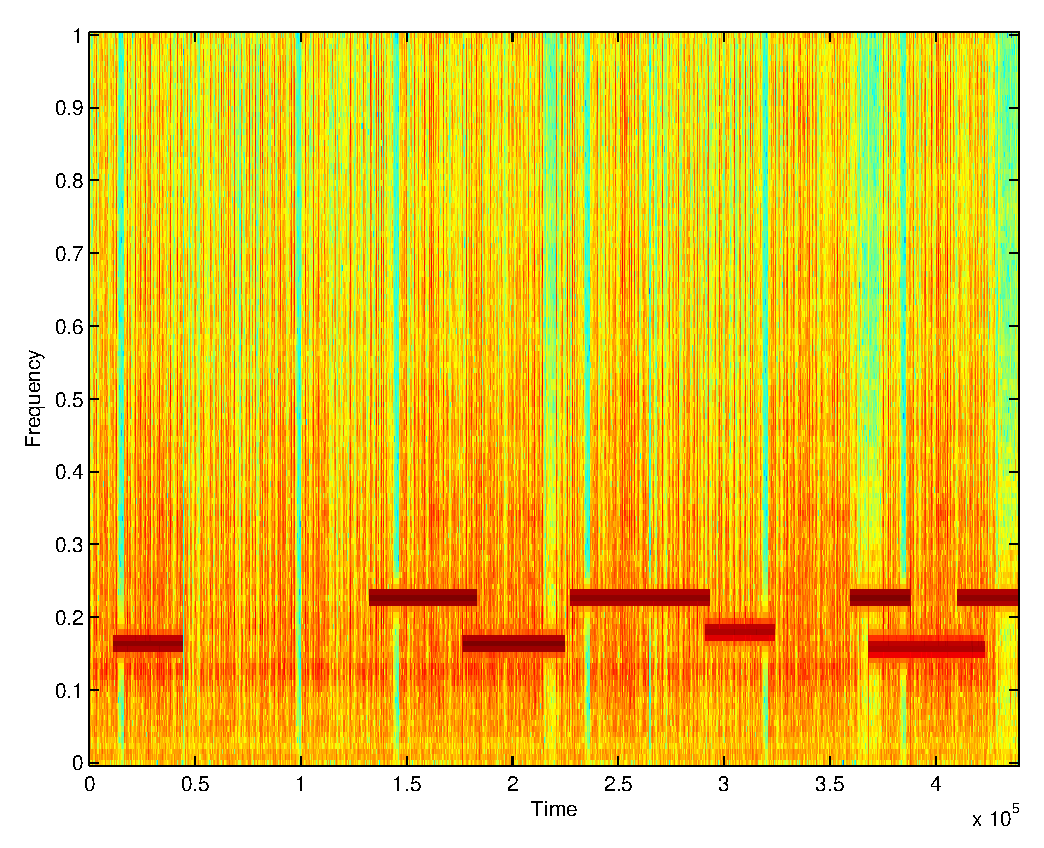
\includegraphics[width=.24\textwidth]{story4_fake.eps}}
 \caption{ A sound scene composed of background and foreground elements 
from several existing scenes }
 \label{fig:teaser}
}
%\teaser{

% The ``\maketitle'' command must be the first command after the
% ``\begin{document}'' command. It prepares and prints the title block.

\maketitle

% Abstract section.

\begin{abstract}

%This paper is abstract (in many ways).
% data-driven - should we add?

A sound scene can be defined as any ``environmental'' sound that has a 
consistent background texture, with one or more potentially recurring 
foreground events. We describe a data-driven framework for analyzing, 
transforming, and synthesizing high-quality sound scenes, with flexible 
control over the various components that make up the synthesized sound. 
Given one or more sound scenes, our system provides well-defined means 
to: (1) identify points of interest in the sound and extract them into
reusable templates, (2) transform sound components independently of the
background and/or other events, (3) continually re-synthesize the 
background texture in a perceptually convincing manner, and 
(4) controllably place event templates over the background, varying key
parameters such as density, periodicity, relative loudness, and spatial
positioning of the components. Our main contributions include: 
techniques and paradigms for template selection and extraction, independent 
sound transformation and flexible re-synthesis; extensions to a wavelet-based 
background analysis/synthesis; and user interfaces to facilitate the various 
phases in our approach. Given this framework, it is possible to completely 
transform an existing sound scene, dynamically generate sound scenes of 
unlimited length, and construct new sound scenes by combining elements from 
different sound scenes.

%We describe a framework for synthesizing perceptually-convincing sound 
%scenes of unlimited length, with fine control over the characteristics 
%and occurrences of individual foreground events and the qualities of the 
%sound scene. Given one or more example sounds, the system can 
%automatically locate and isolate deterministic (sinusoidal) events, 
%transient events, and background textures into reusable templates.  Our 
%framework also allows users to interactively highlight points of 
%interest in the sound for event isolation, manipulate events 
%independently, change the density of events, and even create new sound 
%scenes by combining elements of different source templates.  

%Our general approach models foreground events and background sound 
%separately. We apply  spectral modeling to extract deterministic  
%sinusoidal events and a stochastic residue from the given sound.  The 
%deterministic events are then generated to order, possibly after 
%spectral transformations, using sinusoidal re-synthesis. The 
%stochastic component may also contain non-sinusoidal events, known as 
%\textit{transients}. We generate the stochastic component using wavelet 
%tree learning. The resulting system provides a new paradigm for 
%interactively synthesizing high-quality sound texture with flexible 
%control over the variety and quality of the synthesized sound.

%Citations can be done this way~\cite{Jobs95} or this more concise 
%way~\shortcite{Jobs95}, depending upon the application.
\end{abstract}

% ACM Computing Review (CR) categories. 
% See <http://www.acm.org/class/1998/> for details.
% The ``\CRcat'' command takes four arguments.

%\begin{CRcatlist}
%  \CRcat{K.6.1}{Management of Computing and Information Systems}%
%{Project and People Management}{Life Cycle};
%  \CRcat{K.7.m}{The Computing Profession}{Miscellaneous}{Ethics}
%\end{CRcatlist}
% The ``\keywordlist'' command prints out the keywords.
%\keywordlist
\section{Introduction}
% The ``\copyrightspace'' command must be the first command after the 
% start of the first section of the body of your paper. It ensures the
% copyright space is left at the bottom of the first column on the first
% page of your paper.
%\copyrightspace
Many sound synthesis techniques focus on generating foreground sounds 
such as voices, music, interactions between objects or sudden events that 
attract our attention. These sounds alone do not generally give the listener 
a strong sense of being in a real-world environment where there are many 
background noises as well. The totality of sounds that compose an auditory 
scene, or a sound scene, is the focus of the work described in this paper.  
Existing sound synthesis methods that deal with pre-recorded sound do not 
provide suitable analysis and synthesis techniques for truly flexible ``sound 
scene modeling by example,'' where a sound scene can be composed from selected 
components of different example sounds. 
%This is analogous to the data-driven 
%surface construction approach used in 3D geometric modeling by example  
%~\cite{Funkhouser04}. BETTER ANALOGY: vision? 
From a user's point of view, this process is somewhat analogous to 
using computer vision tools for intelligent scissoring and image 
segmentation ~\cite{Mortensen95,Rother04,Wang05}.

Sound scene modeling by example is the creation of perceptually convincing 
sound scenes based on a set of existing sounds. The generated sound  
should be arbitrarily close to or different from the original sounds, based on 
the user's intention. Naive approaches such as repeatedly playing or combining 
raw segments of original recordings do not sound convincing, while more complex 
sound synthesis methods lack flexibility both in creating scenes and in the 
amount of user control needed.
%The generated sound should be arbitrarily close to or different from the 
%original, so that it can either be perceived as another instance of it or 
%as a completely different scene. Since repeatedly playing the original 
%sound is not convincing, the synthesis should involve some randomness as 
%well as a flexible amount of user control. NOT MAKING SENSE AS A PARAGRAPH.

Given one or more existing sound scenes, our task is to generate from 
these an unlimited supply of non-repeating, perceptually convincing 
sound that can be parametrically controlled to fit the user's 
specifications. Another goal is to provide an automation tool for 
easily modeling and generating sound scenes for 
entertainment (movies, TV, and games), Virtual and Augmented Reality, 
and art projects such as live performances and installations.

Towards this aim, we introduce TAPESTREA: Techniques and Paradigms for 
Expressive Synthesis, Transformation and Rendering of Environmental 
Audio. Our general approach is based on the notion that sound scenes are 
composed of events as well as background sound, which are best modeled 
separately. In particular, we separate a sound scene into the following 
components:\\
(1) \emph{Deterministic events}: composed of highly sinusoidal components, 
often perceived as pitched events, such as a bird's chirp or a baby's cry;\\
(2) \emph{Transient events}: brief non-sinusoidal events, such as footsteps;\\
(3) \emph{Stochastic background}: the ``din'' or residue remaining after the 
removal of deterministic and transient components, such as wind, ocean waves, or 
street noise.

Our system proceeds by analyzing and synthesizing each component separately. It  
applies spectral modeling ~\cite{Serra89} to extract deterministic events 
and a stochastic residue from a given sound. The deterministic events are 
then generated to order, possibly after spectral transformations, using 
sinusoidal re-synthesis. TAPESTREA isolates and extracts transients either before or 
after the spectral modeling analysis. The final stochastic background is 
obtained by removing the deterministic as well as transient events 
from the given sound and filling in the holes left by transient removal. 
Once the background component has been separated, the system dynamically 
generates it using a wavelet tree learning algorithm by Dubnov et. al. 
~\shortcite{Dubnov02}, with significant improvements. Running this algorithm 
on a stochastic background with no sinusoidal components allows the wavelet 
tree learning to operate on the type of data with which it works best.  

Our approach is distinct from existing methods in sound synthesis in that it allows users to:
(1) point at a sound or a part of a sound and request more or less of it in the final scene,
(2) transform that sound independently of the background,
(3) flexibly control important parameters of the synthesis, such as density, periodicity, relative gain, and spatial positioning of the components
(4) construct novel sounds in a well-defined manner.

%  Put this somewhere else maybe:  SMS techniques has been primarily used for 
%  analysis/modeling of foreground musical sounds.  We are the first (and the last probably) to 
%  use it for event separation in texture synthesis.

%Our method also allows users to have control over the characteristics of their synthesized 
%texture. Separating the events provides a framework in which to manipulate events 
%individually, and to request more occurences of some events and less of others in the final 
%texture. It also offers the option or creating new sound textures by mixing the backgrounds 
%and deterministic events from several example textures.

%PLACEHOLDER: our contributions are too numerous to list here, a random sampling:
% observation: separation of foreground events and background din is beneficial
%    - indepedently transform events and background
%    - you can add or remove instances of events
%    - mix events from different sources
%    - better results (we hope) from wavelet
% contribution:
%    - system for doing it
%    - a user interface for building new sound textures

%   1.1 Motivation\\
%   		 - what is a sound texture anyway?\\
%       - "i have this sound texture, I want to produce more of it.
%          and in this way (clarifify)"\\
%       - give sound designers automation tool\\
%   1.2 Our general approach (what we are describing in this paper)\\
%	- we like wavelet tree learning and we like sms\\
%	- we want to realize the future section of wavelet tree, be able to point at 
%components of a sound and ask for more or less of it\\
%	- using sms plus feature based audio classification we gain\\
%	---we can separate out events/foreground\\
%	---we make wavelet tree better because we separate harmonic events, which wavelet tree 
%is not good at handling\\
%	- transform: because we have individual events we can modify and place them 
%independently\\
%	- more control over the textures we synthesize (example somewhere)\\

%CONTRIBUTIONs listed above (not commented out)

The rest of the paper is structured as follows: In Section 2 we describe 
related work, which includes ways for rendering simulated and 
model-based foreground sounds, methods for synthesizing background textures, 
and information on spectral modeling. Section 3 provides an overview of our 
approach along with an example highlighting how it can be used. Section 4 
describes the analysis stage of our framework, section 5 describes the possible 
transformations on events, and section 6 describes the synthesis phase. 
Section 7 provides details about our user interface and section 8 summarizes results 
and contributions. Section 9 describes our conclusions and directions for future work. 


\section{Related Work}

Previous work on synthesizing sound to match a given environment has 
involved simulation or model-based methods for generating interactive 
contact sounds, or the analysis and re-synthesis of existing sounds. 
Tools for sound production also include a range of sound editors. 
%While our work draws on some of these ideas, we focus on the 
%analysis and re-synthesis of environmental sounds.

\subsection{Simulated and Model-based Sounds}

Simulation and model-based sound synthesis techniques are based on physical models of the 
objects, the world, and/or the interactions between these ~\cite{CookBook}. 
Physically based models have been used to generate foreground sounds such as those caused by object interactions, including walking sounds ~\cite{Cook02}, sounds caused by the motion of 
solid objects ~\cite{OBrien01}, complex sounds due to individual objects and gestures 
~\cite{Rocchesso03}, and contact sounds ~\cite{Doel01} such as colliding, rolling, and 
sliding. Aerodynamic sounds ~\cite{Dobashi03} have been rendered using computational fluid 
dynamics. Models of a virtual environment have also been used for effective sound 
rendering ~\cite{Takala92,Tsingos04}.

%Physics based motion-driven synthesis ~\cite{Cardle03, Dobashi03}.

The advantage of simulated and model-based approaches is that given a model, sound can be
directly inferred, synthesized, and transformed by modifying the model parameters. 
However, the requirement of having a model in order to generate sound  makes these methods 
difficult to generalize. Production audio often uses pre-recorded sounds instead of models; it is therefore worthwhile to make the processing of pre-recorded sounds as parametric as possible. 

%this is not what we are doing.

\subsection{Sound Textures}

A sound texture can be described as a sound with structural elements 
that repeat over time, but with some randomness. The sound of rain falling, 
leaves rustling in the wind, or applause are examples of sound textures. 
Textures often form a large part of the background of sound scenes.
Existing work on sound texture synthesis most resembles our goal of synthesizing
entire sound scenes, as a sound texture can be thought of as environmental audio.

Athineos and Ellis ~\shortcite{Athineos03} modeled sound textures composed of
very brief granular events known as \textit{micro-transients}, such as 
fire crackling or soda being poured out of a bottle. 
Zhu and Wyse ~\shortcite{Zhu04} extended their technique to separate 
the foreground transient sequence from the background din in the source 
texture and resynthesize these separately. Both these methods are effective on textures 
that primarily contain micro-transients, but do not generalize well to other sounds. For 
instance, the foreground-background separation misses spectral foreground events, as it does 
not take frequency into account while identifying events.

Miner and Caudell ~\shortcite{Miner97} used wavelets to decompose, 
modify, and re-synthesize sound textures, concentrating 
on the perceptual effects of various transformations. 
%This technique 
%requires some specialized knowledge for obtaining particular results, as 
%the parameters to be manipulated do not directly map to audible sound 
%characteristics. 
Dubnov et. al. ~\shortcite{Dubnov02} also used a wavelet decomposition to 
analyze and generate more of a sound texture. 
%analyze the temporal and spectral structure of a sound texture at various 
%resolutions. 
Their method works well for sounds that are mostly 
stochastic or have very brief pitched portions. However, sounds with 
continuous components, such as a formula-one racecar engine, sometimes 
get chopped up, while rhythmic sounds may lose their rhythm during 
synthesis. The technique is also not suitable for sounds with 
many sinusoidal components, as these are not modeled well by a 
stochastic process.
 
In general, these existing approaches work only for largely stochastic 
sounds and 
do not allow flexible control over the output---either the entire texture is 
transformed or segments are shuffled and concatenated. Hence 
these methods are insufficient for sounds that have various foreground events and 
background playing simultaneously.
Our approach overcomes these limitations by isolating and removing 
pitched sounds, performing modified wavelet tree learning 
~\cite{Dubnov02} on the  
remaining stochastic part, and re-inserting the extracted components 
afterwards. We separate the pitched components from the sound texture 
using spectral modeling, as described in the next section.

%Given an existing ambient/background/environment sound of limited, 
%length, it is possible to synthesize more of the same texture. This 
%method has no prior knowledge of the objects in the environment. 


%       - texture synthesis from existing ambient/background/environment
%         sounds (of limited length)\\
%       - LPC fails (probably)\\
%         --- good for micro-transients\\
%       - dubnov et. al.  (2002)\\
%         --- showed how to take apart and synthesize more of it but...\\
%         --- individual events not good for chopping up, not good for repeating\\
%       - miner and caudell\\
%       - we come in here...\\
%         --- event identification/isolation/transformation/(authentification)
%           (better analysis)\\
%         --- take better advantage of wavelet tree learning \\
%         --- separation of control over background and events
%           (more control during synthesis)\\
%         --- more potential for interactivity\\
%         --- combine many of these approachs + spectral modeling\\
%         --- talk about how our stuff differs\\

\subsection{Spectral Modeling}

Spectral modeling builds on the notion that some components of sound fit a sinusoidal model 
while others are better modeled by spectrally shaped noise. 
The Fourier transform allows us to inspect a sound's spectrum and identify components that 
would best be modeled by sinusoids. These are known as deterministic components; 
subtracting these from the original sound yields the residual or stochastic component that 
ideally contains only noise. 

Serra and Smith ~\shortcite{Serra89} posed the concept of ``sines plus noise'' 
modeling and developed the Spectral Modeling Synthesis (SMS) system, building on the 
original sinusoidal modeling algorithm ~\cite{McAulay86} and applying it to musical sounds. 
Sinuosoidal modeling also enables modification of the original sound before re-synthesis, for 
instance by pitch-shifting and time-stretching.
Other related work on spectral analysis includes alternatives to 
the Fourier transform for estimating the spectra of specific kinds of 
signals ~\cite{Qi02,Thornburg03}. 

Existing tools for spectral analysis and re-synthesis, such as SPEAR ~\cite{Klingbeil05}
and the CLAM library ~\cite{Amatriain05}, allow high-level sinusoidal analysis, 
transformations and re-synthesis. But they do not offer the level of parametric control over 
these stages suitable for analyzing and creating sound scenes. Further, they lack a 
framework for processing transients and stochastic background components.

\subsection{Sound Editors}

Current tools for commercial or home audio production include a range of sound editors. Free 
or inexpensive commercially available software such as Audacity and GoldWave perform simple 
audio production tasks. Midline audio editing systems, including Peak, Logic, and Cubase, are 
geared towards music production and often offer real-time MIDI sequencing capability. At the 
high end are digital audio production hardware/software systems such as Pro Tools, geared 
towards commercial sound production. Most of these products support Virtual Studio Technology 
(VST) plug-ins that perform synthesis algorithms and apply effects such as reverb. However, none of them provides one real-time, extensible, integrated analysis-transformation-synthesis workspace similar to TAPESTREA.  

%\begin{equation}
% \sum_{j=1}^{z} j = \frac{z(z+1)}{2}
%\end{equation}

\section{Example and Overview of our Approach}

The TAPESTREA system starts by loading an existing sound scene, for example, the sound 
of a city street, a factory environment, seagulls by the ocean or children playing in a park.
The duration of the scene may be 5--15 seconds or longer. Sound events in the park scene, 
for example, may include (1) children yelling, (2) 
a ball bouncing, and (3) geese honking in a nearby pond. The background texture might 
consist of the general din of the surroundings. No 
{\it a priori} knowledge of the existing sound is needed; users can interactively 
direct its operation for specific results.  Also, it is possible for the system to operate
unsupervised from beginning to end given a set of parameters.

\begin{figure}[h]
\centering
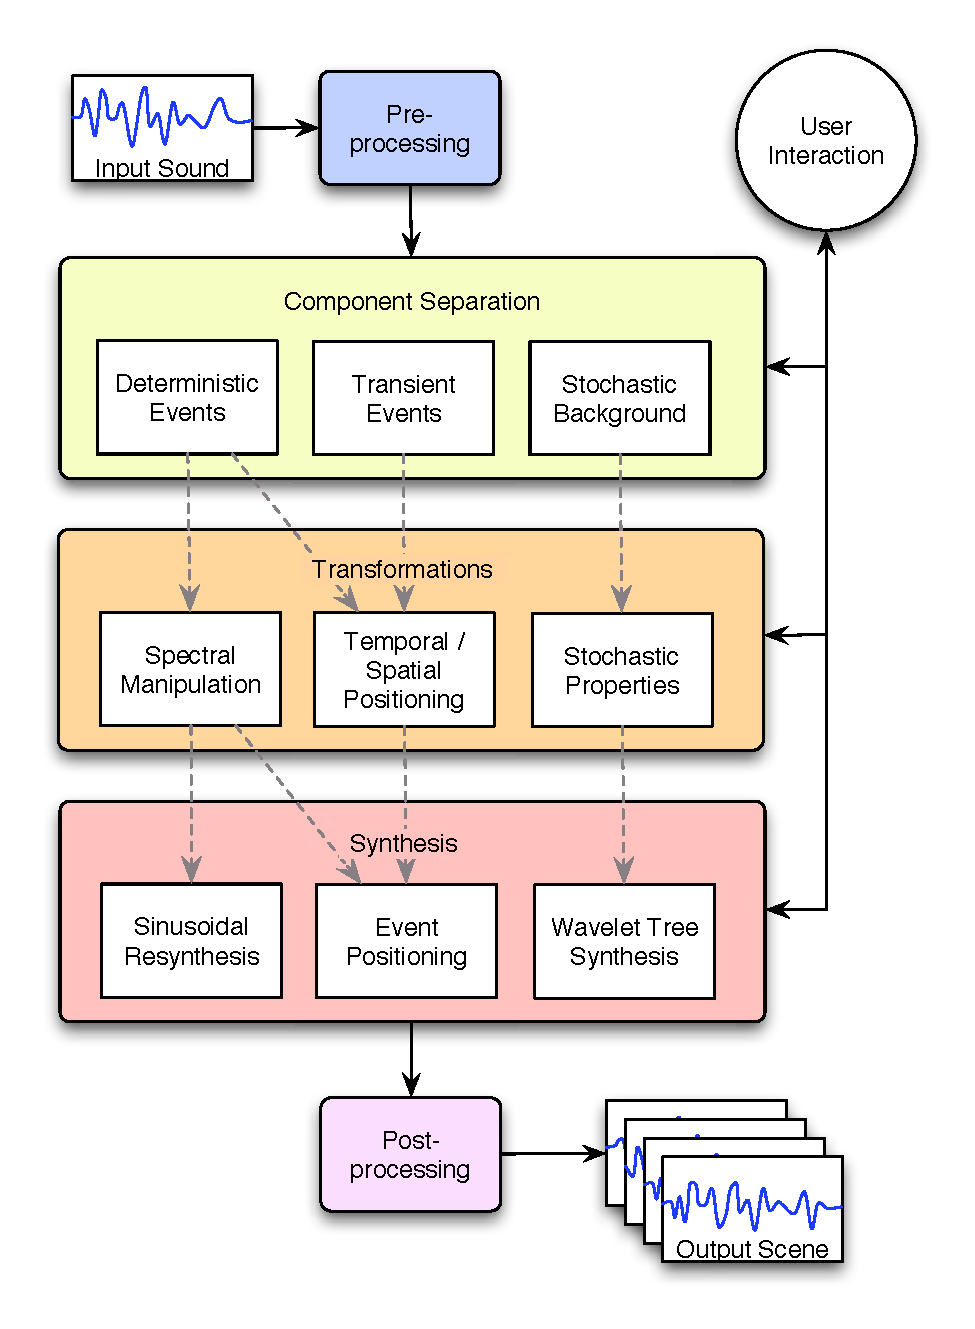
\includegraphics[width=.95\columnwidth]{ourpipeline2.eps}
\caption{Stages in our pipeline: The preprocessed sound is analyzed to enable component separation. These components undergo optional transformations before they are individually synthesized and combined to produce the final sound.}
\label{fig:pipeline}
\end{figure}

Figure \ref{fig:pipeline} depicts the phases in the TAPESTREA pipeline. The existing sound scene first
undergoes a basic preprocessing phase involving sample-rate/data-depth 
conversion as needed, channel information, DC blocking and data normalization. Next, it passes through the 
analysis phase, where the sound is separated into deterministic (children yelling, geese honking), 
transient (ball bouncing) and stochastic background (general din) 
components based on the analysis parameters. Each component can be played back separately 
and stored as a template for future use. For example, one bounce of the ball can 
be stored as a transient template while individual yells can be saved as deterministic event 
templates. In the transformation and synthesis phase, the system or user parametrically specifies how to construct the output sound scene. Transformations can be applied to individual 
templates and these templates can be combined in specified ways to generate a complete sound scene. 
For instance, the output sound scene can consist of a repeatedly bouncing ball and many children yelling 
at different pitches and times over a continuous general din, to simulate a 
children's game with enthusiastic spectators in a park without geese. The output sound scene can in fact   
include templates from any number of existing sound scenes, making it possible to add a referee's whistle, 
for example. The synthesized sound scene can be written to a file or played continuously in real-time 
for as long as needed. TAPESTREA also includes a graphical user interface for interactive control 
of the analysis, transformation and synthesis parameters. The following sections provide more in-depth 
information on the processing phases and the user interface. 

%\subsection{Analysis}
%The system starts with an existing sound scene, which we will refer to as the
%\textit{template}.  An example template may be the sound of a city street, a factory 
%environment, children playing in a park, seagulls by the ocean, a sporting event, or any other
%ambient or semi-ambient sound.  The duration of 
%the template may be around 10-15 seconds or more, depending on the
%content of the sound.  Sound events in the park template, for example, 
%may include (1) children yelling or talking, (2) clearly audible 
%conversations close to the listener,  (3) children clapping (4) babies 
%crying, and (5) geese honking in a nearby pond. Background textures 
%might include indistinct chatter of people in the park, leaves rustling 
%in the wind, and the general hum of the surroundings.

%No \textit{a priori} knowledge about the existing sound is necessary, 
%though users may (interactively) direct the analysis and synthesis in 
%ways that are specific to the content of the sound and the desired output - 
%for example ``pointing out'' part(s) of the sound to extract or segment.

% Parameters in the interactive mode can also be automated as 
% time-varying parameters in simple scripts, maybe.

%Once a template sound is loaded into the system, the system prepares the template 
%through a basic preprocessing stage (sample rate/data-depth conversion as needed, channel information, data %normalization).
%sub-band correlation for stereo or 
%multi-channel data), and also extracts basic audio features (see section 4), which may serve as hints in the analysis stage.
%Next, the sound template undergoes analysis (sinusoidal modeling, 
%classification, segmentation), which performs the following tasks:
%(1) It isolates \textit{deterministic}, foreground events (i.e. close-up voices, geese).  They are 
%stored as event templates, which can be transformed and
%reused in the synthesis stage.  Statistics about their frequency 
%of occurence are also gathered and stored.
%(2) The analysis also isolates the background texture (general ``hum'' of the surroundings,
%indistinct chatter, rustling leaves, etc.)  The component of the sound is said to be 
%\textit{stochastic}.
%(3) It also segments out brief non-sinusoidal events that stand out from the din. These are called %\textit{transient events}.  The user can listen to each component, and also 
%``fine-tune'' the isolation by selecting time or frequency ranges and analysis thresholds as needed.  The %analysis stage is described in detail in Section 4.

%Heading in the Transformation stage, we now have: (1) ``deterministic'' 
%individual events, isolated in time and frequency from the background and 
%other events, (2) ``stochastic'' background sound texture, and (3) 
%potential ``stochastic-lifted'' events.

%\subsection{Transformation/Synthesis}
%During transformation, the system or user parametrically specify how to 
%construct and synthesize the output sound scene.  For foreground
%events, transformations include high-fidelity frequency/magnitude-warping, 
%time-stretching, and transformations that control the temporal and spatial 
%density of event instances.  For background textures, it is possible to parametrically
%alter the ``similarity'' of the sound to the original template.

%For example, if we take a single ``child yelling'' event template from our 
%street scene, we make different instances of the event with varying 
%loudness, frequencies and durations.  We can then specify for them to occur 
%according to some probability, or as a group (child yelling at different 
%pitches and times to sound like many children).  Furthermore, we can pan 
%each instance differently so that it is perceived as originating from a 
%different point in space. The user can experiment with each of these and 
%preview the result before the final reconstruction / synthesis stage.  
%Transformations on events and background are discussed in Section 5.

%(TODO: need to show scripting language or user interface here or earlier)

%The reconstruction / synthesis stage takes event and background templates,
%and produces the output texture according to specification.
%The stochastic background texture is repeatedly decomposed and 
%recomposed (using wavelet tree learning) into new,
%perceptually similar, non-repeating stochastic background textures, 
%which are layered with the foreground of deterministic events.  From the 
%original park sound template, it is possible to generate an arbitrary length 
%sound scene with similar background and distribution of events.  Also, the 
%loudness, frequency-content, density, and spatialization of each 
%component can be controlled and modified independently.  From the same 
%template, we can thus generate a new sound scene that gives the impression 
%of a park with many more children, or that of a less crowded area with more geese 
%than people. We can also vary the parameters dynamically to gradually transform 
%from one to the other.

%TAPESTREA includes a graphical user interface for performing analysis on 
%multiple sounds, and transforming and resynthesizing the components to 
%create new sound scenes. Waveform, spectrum and spectrogram displays in 
%the analysis view allow users to easily select events to extract. The 
%transformation/synthesis view depicts the separated components as 
%templates and allows the user to manipulate each template separately or 
%group multiple templates together. The interface also provides a means 
%for controlling analysis, transformation and synthesis parameters in 
%real-time. 

%what a messy pile of words.  YES!!

%The Pipeline

%   3.1 pipeline\\
%       --- input\\
%       --- analysis, event separation\\
%       --- transformation\\
%       --- synthesis\\
%       --- output\\
%       --- control points\\
%   3.2 list of contribution\\


\section{Event Identification and Isolation}

The first step in our framework is to identify and separate foreground events from 
background sound / noise. Foreground events are parts of the scene that are perceived as distinct occurrences, and include both \emph{deterministic events} (the 
sinusoidal or pitched components of a sound) and \emph{transient events} (brief bursts 
of stochastic energy). Removing these leaves us with the \emph{stochastic background}. 

%\subsection{Preprocessing}

%We are considering several ways of preprocessing the given sound 
%texture to enhance deterministic and transient event extraction. One strategy is to bandpass-filter 
%the sound and perform event detection separately on each subband. This 
%could be useful because what is perceived as an event may differ according 
%to the spectral range in which it takes place. For example, high-frequency
%sounds
%(specific range?)
%are easier to detect than low-frequency sounds of 
%the same magnitude (I think). So processing each subband separately allows 
%for better fine-tuning of the event detection / tracking parameters.
%
%Another form of preprocessing is to intelligently segment the given sound 
%texture using the MARSYAS framework. Each segment could then be processed 
%separately. Since each segment is a contiguous-time clip with uniform 
%features, doing this could also aid event identification.
%
%The thing we actually do is block DC.
%
%\subsection{Classification}
%
%PROBABLY DITCH CLASSIFICATION, AND LEAVE IT FOR FUTURE WORK.
%As described earlier, classification of 
%sounds can give us hints on the appropriate parameters or techniques to use for event detection and 
%tracking. We can classify based on various features, including power, spectral centroid and 
%rollof, spectral flux, zero crossing rate, and Mel-Frequency Cepstral Coefficients. For 
%domain-specific tasks, features such as Parametric Pitch Histogram, and Beat/Periodicity 
%Histogram can be calculated and used. These features also aid segmentation of the original 
%sound, as described in Section 4.1.

\subsection{Sinusoidal Modeling}

To identify deterministic events, our system performs sinusoidal analysis based on the 
spectral modeling framework. The input sound scene is read in as possibly overlapping 
frames, each of which is transformed into the frequency domain using the 
FFT and processed separately. The maximum and average 
magnitudes of the spectral frame are computed and stored. The following 
steps are then repeated until either a specified maximum number (N) of peaks 
have been located or no more peaks are present:

%The lowest frequencies in the spectral frame are eliminated to avoid 
%artifacts from the transform and windowing.
%(kind of ambiguous)(why?)

(1) The maximum-magnitude bin in the frame, within the specified frequency range, is 
located.\\
(2) If the ratio of its magnitude to the average magnitude of the frame is 
below a specified number, it is assumed to be noise and we deduce that no 
more peaks are present.\\
(3) If its magnitude is above a specified absolute threshold, it is added as a 
sinusoidal peak and the bins it covered are zeroed out in the analysis frame.
\begin{figure}[h]
\setlength\textfloatsep{0pt}
\setlength\abovecaptionskip{0pt}
\setlength\belowcaptionskip{0pt}
\centering
   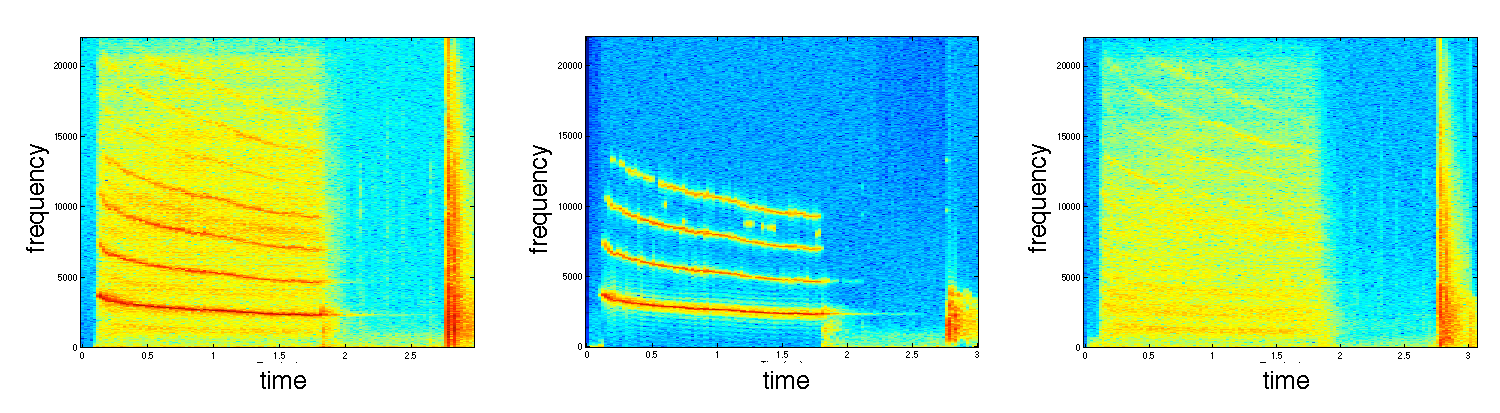
\includegraphics[width=.48\textwidth]{fireworks3.eps}
%  \subfigure[]{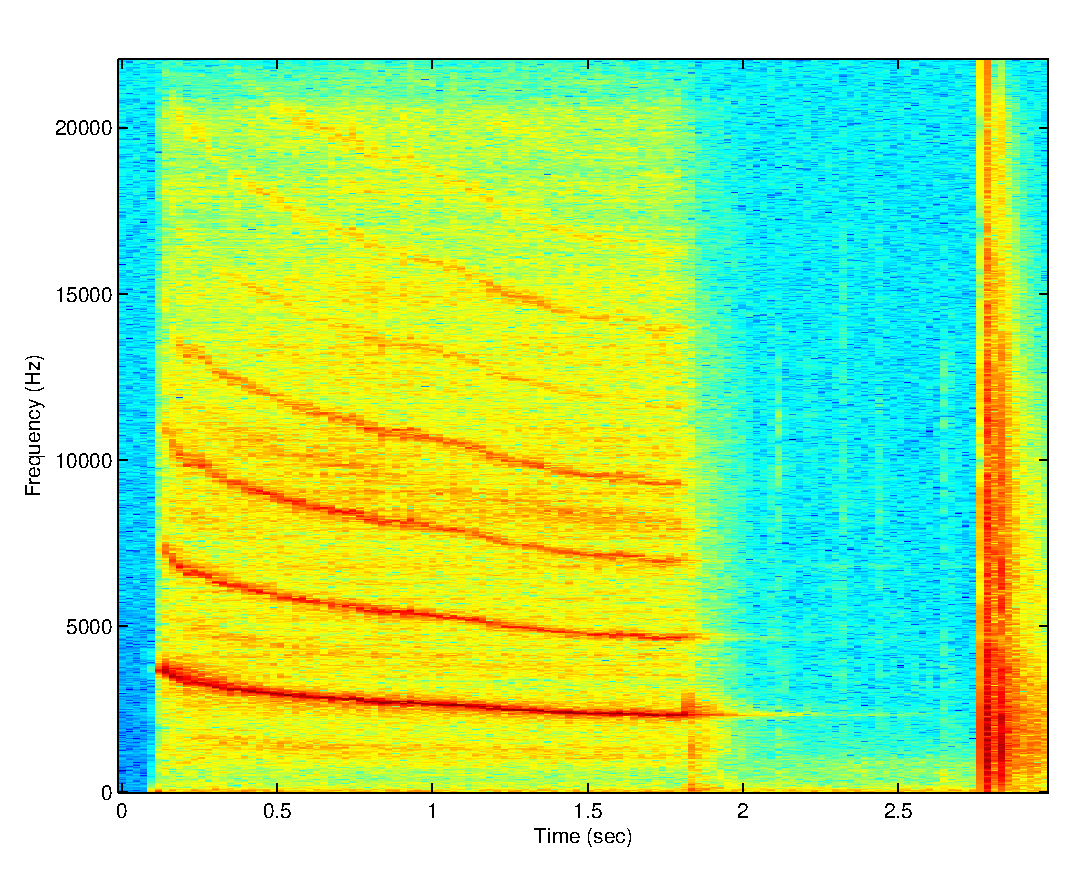
\includegraphics[width=.155\textwidth]{firework.eps}}
%  \subfigure[]{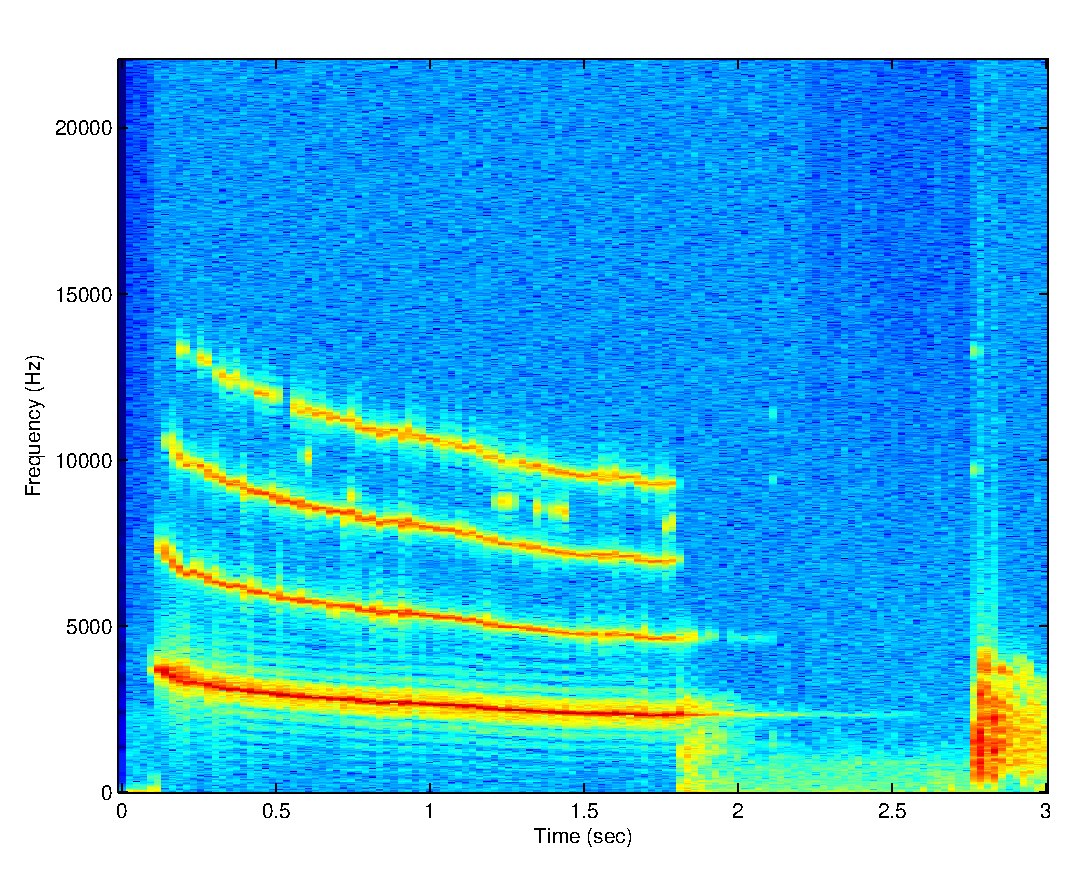
\includegraphics[width=.155\textwidth]{fireworktracks2.eps}} %.7159*.22=.1575
%  \subfigure[]{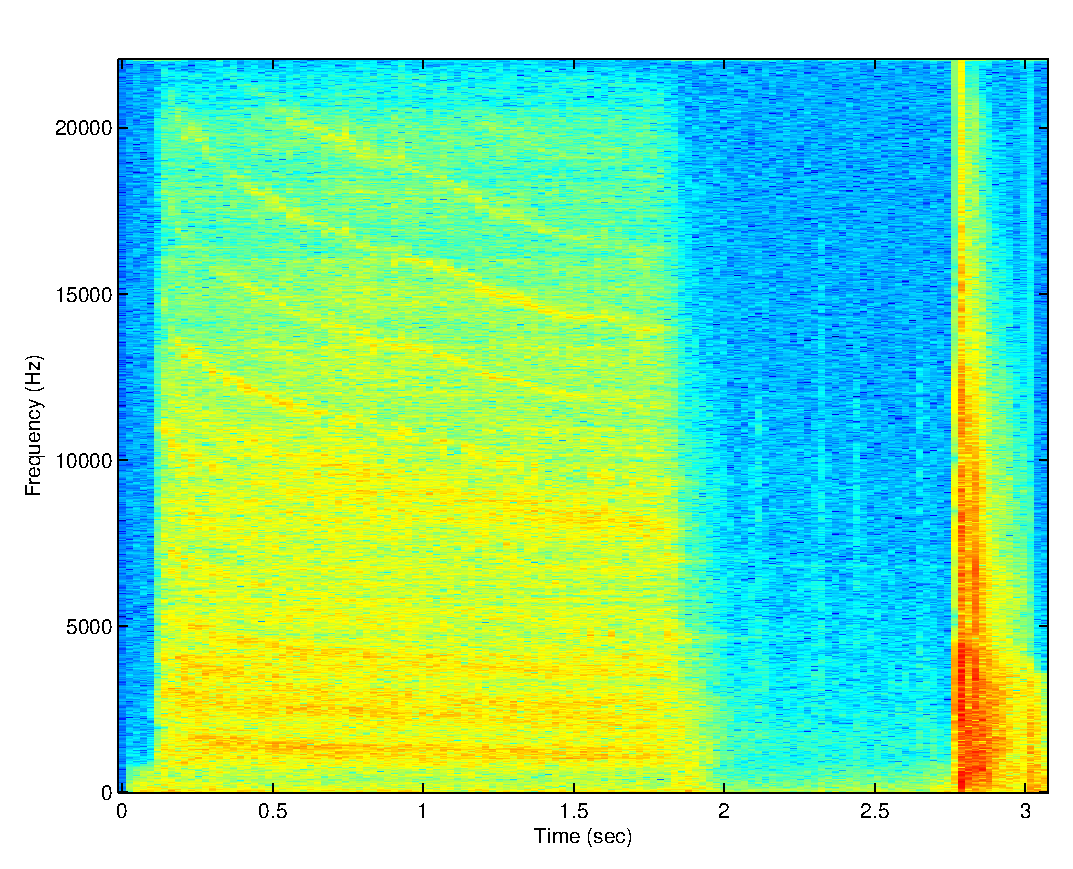
\includegraphics[width=.155\textwidth]{fireworkres2.eps}}
\caption{Separating sinusoidal tracks from stochastic residue: (a) original sound; 
(b) sinusoidal tracks; (c) residue}
\label{fig:sines}
\end{figure}

The sinusoidal peaks and FFT frames can also be pre-computed. In this case, all peaks in 
a frame are found by locating bins where the derivative of the spectrum changes from 
positive to negative. The peaks for each frame are stored in decreasing magnitude order.
During run-time, the top N peaks that satisfy any frequency and threshold 
bounds are selected per frame in preparation for peak matching. 

Once the top N peaks in all the frames have been collected, our system matches peaks 
from frame to frame if they occur at sufficiently similar frequencies. 
Over time this yields \emph{tracks} of peaks lasting across frames. The 
matching and updating of tracks takes place in the following way:

(1) Each existing track from previous frames selects a current frame peak that is 
closest to it in frequency. If the difference in 
frequency is above a reasonable amount of change, that track is considered dormant 
and the selected peak remains unmatched.\\
(2) All remaining current peaks that have not been matched to a track are 
added as new tracks, and all existing tracks that have not found a 
continuation are removed if they have remained dormant for several frames.\\
(3) Tracks that continue across several frames are retained. 

Finally, TAPESTREA can automatically group related tracks ~\cite{Ellis94,Melih00} 
to identify events. A track is judged to belong in an existing group if it has a 
sufficient time-overlap with the group and its frequency is harmonically 
related to that of a track in the group, its frequency and amplitude 
change proportionally to the average frequency and amplitude of the 
group, or it shares common onset and offset times with the group average. If a track 
appears to belong in multiple groups, these groups are merged. While the grouping could 
benefit from a more sophisticated algorithm and/or machine learning, it can currently be 
fine-tuned for specific sounds by manipulating the error thresholds (set by default to the 
most generally effective values). Groups that last over a minimum time span are considered 
deterministic events. 

Deterministic events are then represented as a collection of sinusoidal tracks. Each 
event is defined by a list of tracks, as well as 
a history of the frequency, phase and magnitude of each track 
over its frames and the times of that track's onset and completion. 

The residue, or the sound with deterministic components removed, is extracted 
after the sinusoidal tracks have 
been identified. Our system eliminates each peak in a sinusoidal track from the corresponding 
spectral frame by smoothing down the magnitudes of the bins beneath the peak. 
It also randomizes the phase in these bins. Figure ~\ref{fig:sines} shows sinusoidal 
separation results. 

\subsection{Transient Detection and Separation}

Transients are brief stochastic sounds with high energy. While a sinusoidal track 
looks like a near-horizontal line on a spectrogram, a transient 
appears as a vertical line, representing the simultaneous presence of information 
at many frequencies. Transients are usually detected in the time domain by observing 
changes in signal energy over time ~\cite{Verma98,Bello05}. 
In our framework, the entire sound file is processed 
using a non-linear one-pole envelope follower filter with a sharp attack and gradual 
decay to detect sudden increases in energy. Points where the derivative of the envelope 
is above a threshold mark transient onsets. 
\begin{figure}[h]
\setlength\textfloatsep{0pt}
\setlength\abovecaptionskip{0pt}
\setlength\belowcaptionskip{0pt}
\centering
   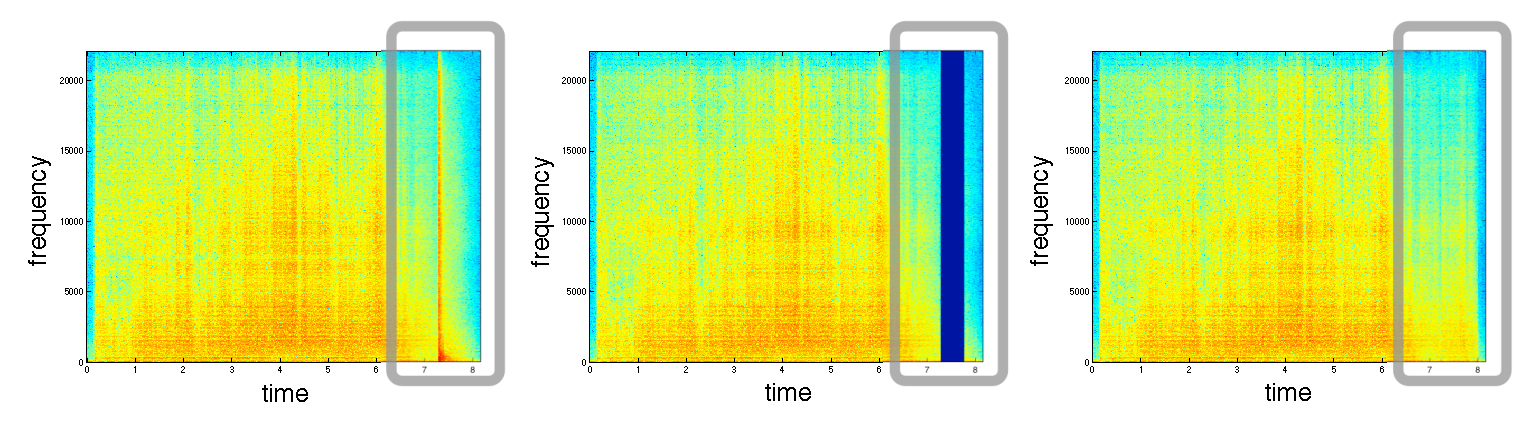
\includegraphics[width=.48\textwidth]{transient3.eps}
%  \subfigure[]{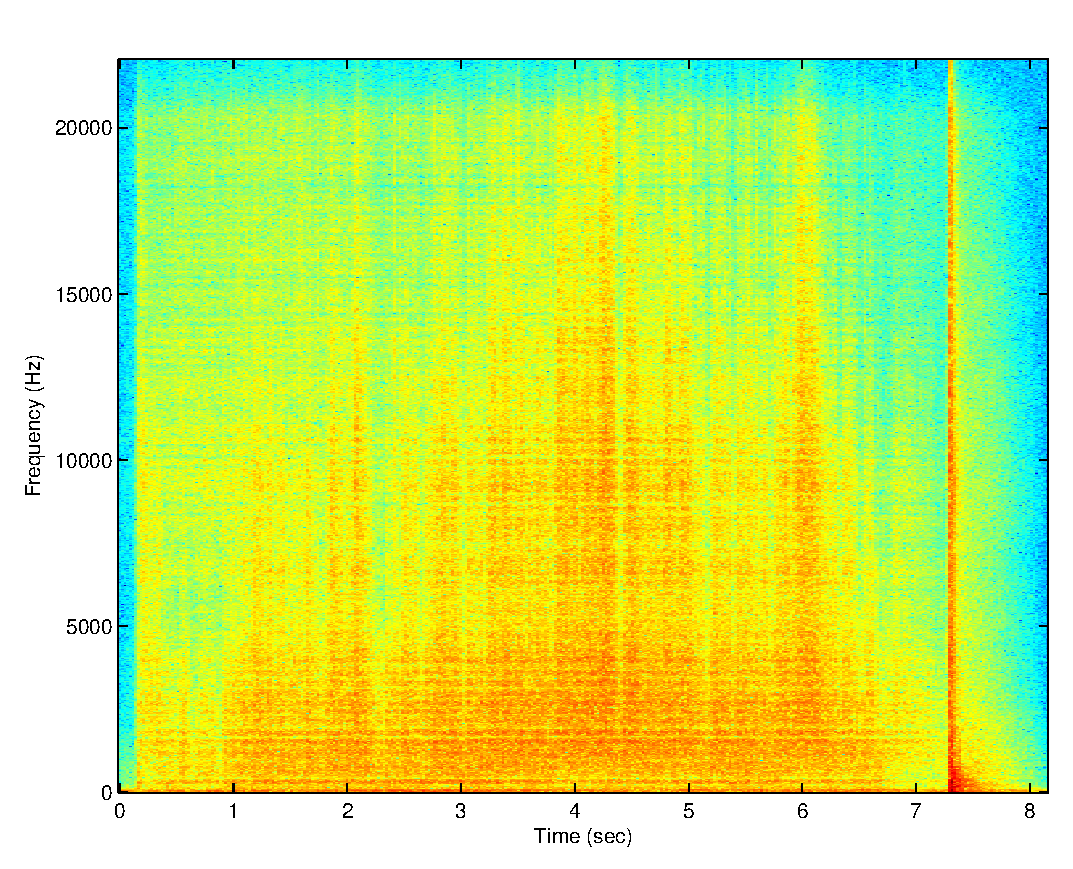
\includegraphics[width=.155\textwidth]{transient.eps}}
%  \subfigure[]{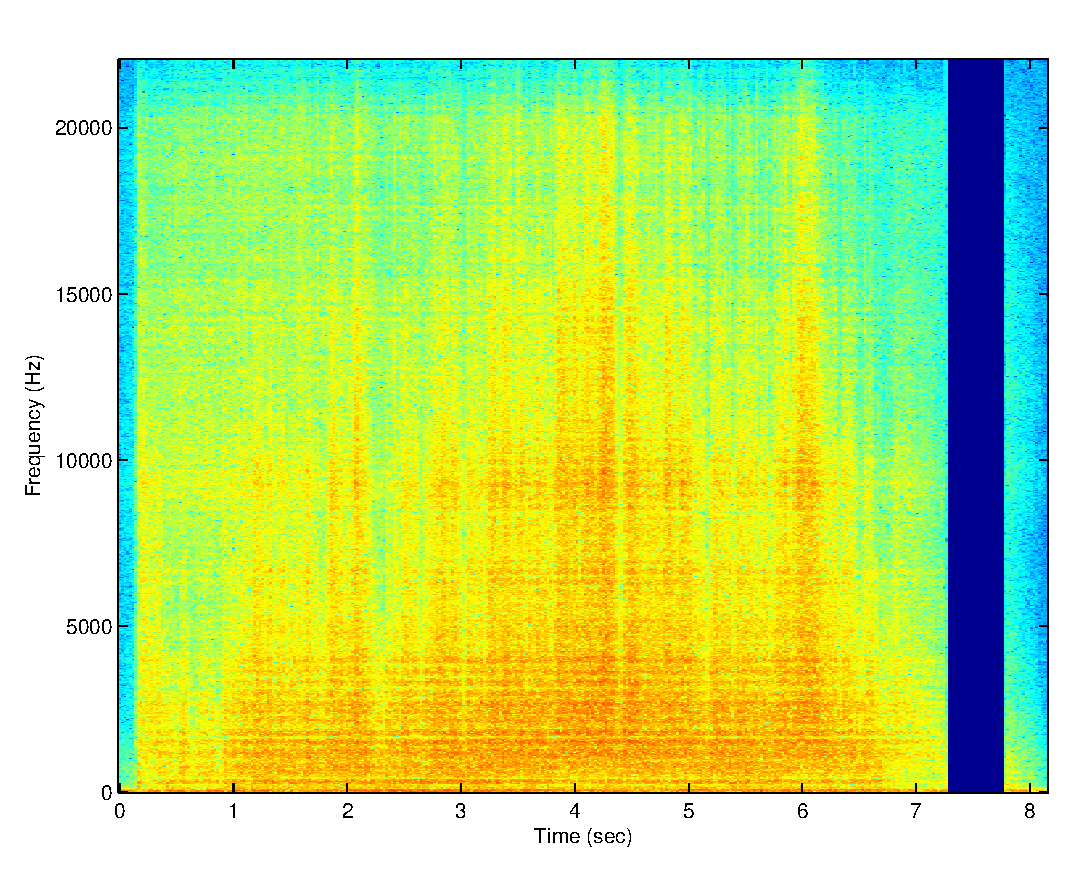
\includegraphics[width=.155\textwidth]{transient-.eps}}
%  \subfigure[]{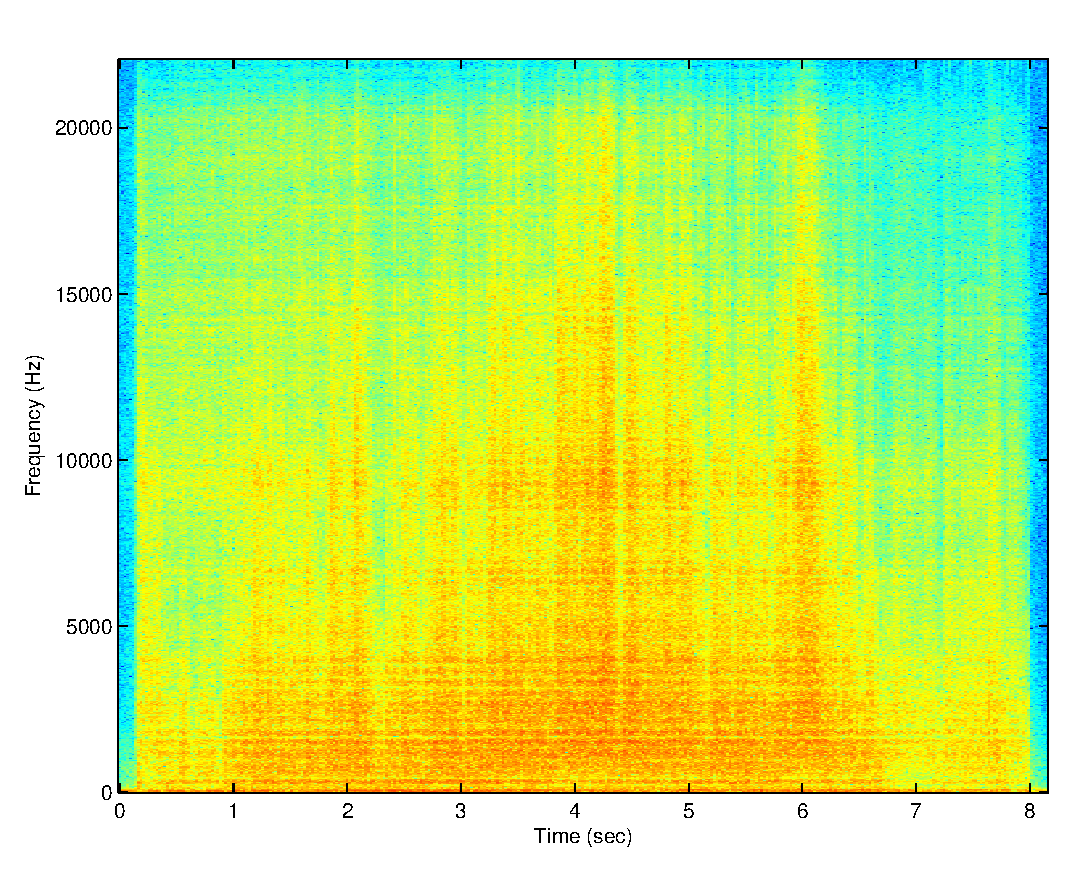
\includegraphics[width=.155\textwidth]{transient+.eps}}
\caption{Transient removal and hole filling: (a) fireworks with pop (at 7.2 sec); (b) 
fireworks with pop removed; (c) fireworks with hole filled}
\label{fig:transient}
\end{figure}

Transient events, by definition, are not well represented by sinusoidal tracks as they 
contain many different frequencies. They can instead be modeled by peak picking in the 
time domain ~\cite{Verma98}, as a sort of dual of the deterministic component. 
However, they are generally brief enough and continuous enough to be 
stored as raw sound clips that can be directly replayed or processed as needed; 
this is how we represent them. 

Detected transients are removed, and the resulting ``holes'' are filled by applying the 
wavelet tree learning algorithm. 
The nearest transient-free segments before and after a given transient event are 
combined to estimate the probable background that should replace it. Wavelet tree 
learning then generates more of this background, which is overlap-added into the original 
sound to replace the transient. The residue from the sinusoidal analysis, with transients 
removed in this way, is saved to a file and used for stochastic background generation in the 
synthesis phase. Figure ~\ref{fig:transient} demonstrates the hole-filling. 

%\subsection{Event Representation}

%Deterministic events are represented as a collection of sinusoidal tracks. For each 
%event, we have access to a list of tracks, as well as 
%a history of the frequency, phase and magnitude of each track 
%over its frames and the times of that track's onset and completion. 
%An extension based on this information would 
%be to identify sinusoidal tracks that move in similar ways across the same 
%frames, and group them as a single event or object.

%Transient events, by definition, are not well represented by sinusoidal tracks as they 
%contain many different frequencies. They can instead be modeled by peak picking in the 
%time domain [Verma], as a sort of dual of the deterministic component. 
%However, transient events are generally brief enough and continuous enough to be 
%stored as raw sound clips that can be directly replayed or processed as needed; 
%this is how we represent them. 
%texture, it is isolated in both time and frequency range, and stored as frames of time-varying
%Fourier spectra.  This representation is not as flexible as sinusoidal tracks but represents
%transients better, since they tend to be more noisy than deterministic events, and is amenable
%to spectral transformations.

\section{Transformations}

Going into the Transformation stage, we now have deterministic event 
templates isolated in time and frequency from the 
background, stochastic background sound texture, and transient events.
Now the system or user parametrically specifies how to 
construct and synthesize the output sound scene(s). The deterministic 
events, transient events and background are modeled and transformed 
separately. The power of the parametric model comes from the 
fact that each transformation is applied independently of others, and each component is 
modified independently of other components. 
Since individual events are represented separately, our system also uses 
probability/statistics to model the overall density of many instances of the same event. 
Furthermore, the representation allows individual event panning across speakers and is 
amenable to external algorithms for spatially positioning events. 

\subsection{Event Transformations}

\textbf{Frequency/magnitude-warping} --- By stretching or compressing spectral
data, we can respectively raise or lower the frequency content of a sound without 
affecting its duration.  For deterministic events with sinusoidal tracks, 
TAPESTREA linearly scales the frequency at each point in the track, 
giving high fidelity frequency warping for almost any factor (limited by our 
range of hearing). For transients, it uses a standard phase vocoder ~\cite{Dolson86} to 
similarly scale the frequency for each frame.
%For transient events, for which there is (more or 
%less) only the raw spectral data, the spectrum of each will need to be 
%shifted and interpolated (cite phase vocoder), and stretching by factor > 
%2.0 may produce artifacts.  
For any event instance, the magnitude (gain) can be scaled uniformly.
%or according to frequency.

\textbf{Time-stretching} --- The track-based representation of deterministic events allows us 
to robustly change the duration of each track by almost any factor without 
producing artifacts. The duration of a deterministic event is increased or 
decreased by scaling the time values in the time-to-frequency trajectory of its track. 
Both time-stretching and frequency-warping can take place in 
real-time for deterministic events. Time-stretching for transients once again uses a phase 
vocoder to stretch or shorten the temporal overlap between frames.  
%For events with sinusoidal tracks, we can modify the 
%track's time-to-frequeny trajectory to increase or decrease the duration 
%independent of the frequency.  For track-based representation, it is 
%robust to change the duration by almost any factor without producing 
%artifacts.  For example, (imagine that you) see figure below.  For 
%transient events, a new frame-based trajectory can be computed, which 
%will be overlap/added to produce time-stretching. 

%Statistics???

\textbf{Temporal placement} --- TAPESTREA allows placement of an individual event in time, either explicitly or using 
a probability distribution for repeating events.  
%Explicitly, it is possible to 
%script 
%the occurrences of a particular event and apply other
%transformations independently on each event instance. 
Explicitly, a particular instance of an event can be placed on a timeline by specifying its onset time. The timeline 
may also include other event instances as well as background sound. Transformations can be applied on individual 
objects both before and after placement in time. 
%An alternative is to specify a probability distribution, 
%such as Poisson.
%For repeating events, an alternative is to specify a mean event density and a probability 
%distribution 
%such as Poisson, selected according to the desired periodicity of the repetition. This 
%allows more automated event placement. 
For repeating events, an alternative is to specify a mean event density and desired 
periodicity of repetition, and use a Gaussian or other probability distribution to automate 
event placement according to these parameters.

%\textbf{Spatial positioning} --- While not the focus of this research, it 
%is straightforward to spatially position or move individual events in world 
%coordinates.
%Explicitly place (or provide trajectory for) an 
%event instance in space (in world coordinates), and assign a particular 
%spatialization effect by providing something similar to an impulse response
%for the space.  The system can place an event instance any where in world
%space (no occlusions), and calculate for distance attenuation, panning across
%any number of output audio channels, and spatialization if an impulse reponse
%is provided.  NOT THE FOCUS OF THIS RESEARCH.

%\subsubsection{Group Control}

%\textbf{Density} - Specify density, or texture of a group of events; parameters include 
%number of event instances and a probability distribution.  While it's possible to achieve
%this control using temporal placement of individual event instances described previously,
%this offers a more globally-aware control of a sound ``crowd''.  This lends to easier
%control and more potential for system optimizations for a large number of sound sources,
%such as in Tsingos et. al.  Also, the size of the group can be varied dynamically. 
%(ui or example)

%\textbf{Spatial density} - Specify how to distribute group in space.  
%(need interaction here).

\subsection{Stochastic Background Transformations}

In addition to the panning and volume scaling available to all templates, 
the system also provides real-time or 
pre-determined control over the similarity between an extracted background 
and the synthesized background generated from its template.
The similarity or randomness is governed by the parameters to the wavelet 
tree learning algorithm described in section 6.2. Also, the generated background 
can play for any arbitrary amount of time.
%\textbf{Magnitude-warping and panning} - Similar to transient events' frame-based 
%warping - modify the frequency/magnitude of the background texture (using spectral
%modeling).  This can applied either before or after the stochastic modeling.

%\textbf{Time-stretching} - Slow down or speed up the background characteristics, without 
%changing the pitch.

%\textbf{Similarity to original sound} - Modify how similar the new generated background
%will be to the original background.  A lower index of similarity will allow more randomness
%in the synthesized texture.
% - by modify parameters to wavelet tree\\
%--- threshold / randomness (see below)\\
%- synthesis parameters (LPC for micro-transient)\\

%\textbf{Density}\\
% - some metric of stochastic density.\\

\section{Synthesis}

Based on the specified transformations, TAPESTREA synthesizes a sound 
scene to fit the user's preferences. The background 
component and the events are synthesized separately and combined to produce the 
final scene. Although we discuss transformation and synthesis in separate sections for 
clarity, these two aspects are very closely related. For example, components can be 
transformed in certain ways even while they are being synthesized. 
%probability model?

\subsection{Event Synthesis}

The deterministic events are synthesized from their representative tracks with 
sinusoidal re-synthesis, taking into account any specified transformations. 
The system linearly interpolates frequency and magnitude 
between consecutive frames before computing the time-domain sound from 
these. 

Transient events can be directly played back after any 
desired magnitude changes, panning and periodicity or density parameters 
have been specified. If a frequency-warping or time-stretching factor is also specified, the 
event is analyzed and synthesized through a phase vocoder accordingly.

Events can be placed in a synthesized texture according to their 
distribution in the original texture, as shown by Zhu and Wyse 
~\shortcite{Zhu04}. In our system, the user can request more instances of a 
certain type of event or less of another, for a customized sound scene. 
%For example, a view of the spectral domain over time shows 
%distinct peaks, or events, that the user can select. 
An event can also be 
synthesized and played in isolation so that the user can listen to it 
before deciding its role in the final scene.

%example and figure

\subsection{Stochastic Background Generation}

The background is generated using an extension of the wavelet tree 
learning algorithm by Dubnov et. al. ~\shortcite{Dubnov02}. In the original 
algorithm, the background component saved from the analysis phase is 
decomposed into a wavelet tree where each node represents a wavelet 
coefficient, with depth corresponding to resolution.  The wavelet 
coefficients are computed using the Daubechies wavelet with 5 vanishing 
moments. A new wavelet tree is then built, with each node picked 
based on the similarity of its ancestors and its first k predecessors 
(nodes at the same depth but associated with earlier time samples) to 
corresponding sequences of nodes in the 
original tree. The learning algorithm also takes into account the amount of 
randomness desired.

We added the option of incorporating randomness into the first step of 
the learning and modified k to be a fraction of the total number of 
nodes at the current depth, instead of a fixed number. We also found 
that we can avoid learning the coefficients at the highest resolutions, 
without perceptually altering the results. Since the wavelet tree is binary, every additional 
level learned approximately doubles the learning time. Skipping the highest level learning
layers decreases this time by close to half. 
This optimization allowed us to build a real-time version of the wavelet tree analysis and synthesis. 
In addition, interactive control over the learning parameters allows 
users to immediately observe the effects of changing specific parameters, 
and to adjust them accordingly without restarting the process multiple times. 
The wavelet tree learning also works better with the separated stochastic background 
as input since the harmonic events it would otherwise garble have been removed. 
%SAY HOW MUCH FASTER.

%(TODO: fix this)
%- wavelet tree learning works better because we have already separated out 
%what wavelet tree is not good at handling - harmonic events.

\subsection{Putting It All Together}

% The background and events are mixed. 
% At this point the user can sit back and enjoy 
% the display, or interactively fine-tune it, 
% depending on the degree of involvement with which 
% he is most at ease.    
%FIX THIS.  SAY THAT WE CAN
%SYNTHESIZE INFINITE BACKGROUND USING THE WAVELETS,
%AND ADD IN PREVIOUSLY EXTRACTED EVENTS.  CRAFT, 
%SCULPT, DRIVE FROM ALGORITHM (GAME OR ANIMATION),
%ETC.
%Unofficially known as abuser interface.
%figure goes here.  it looks like this:
%... (each dot is a track)
\begin{figure*}[t]
\centering
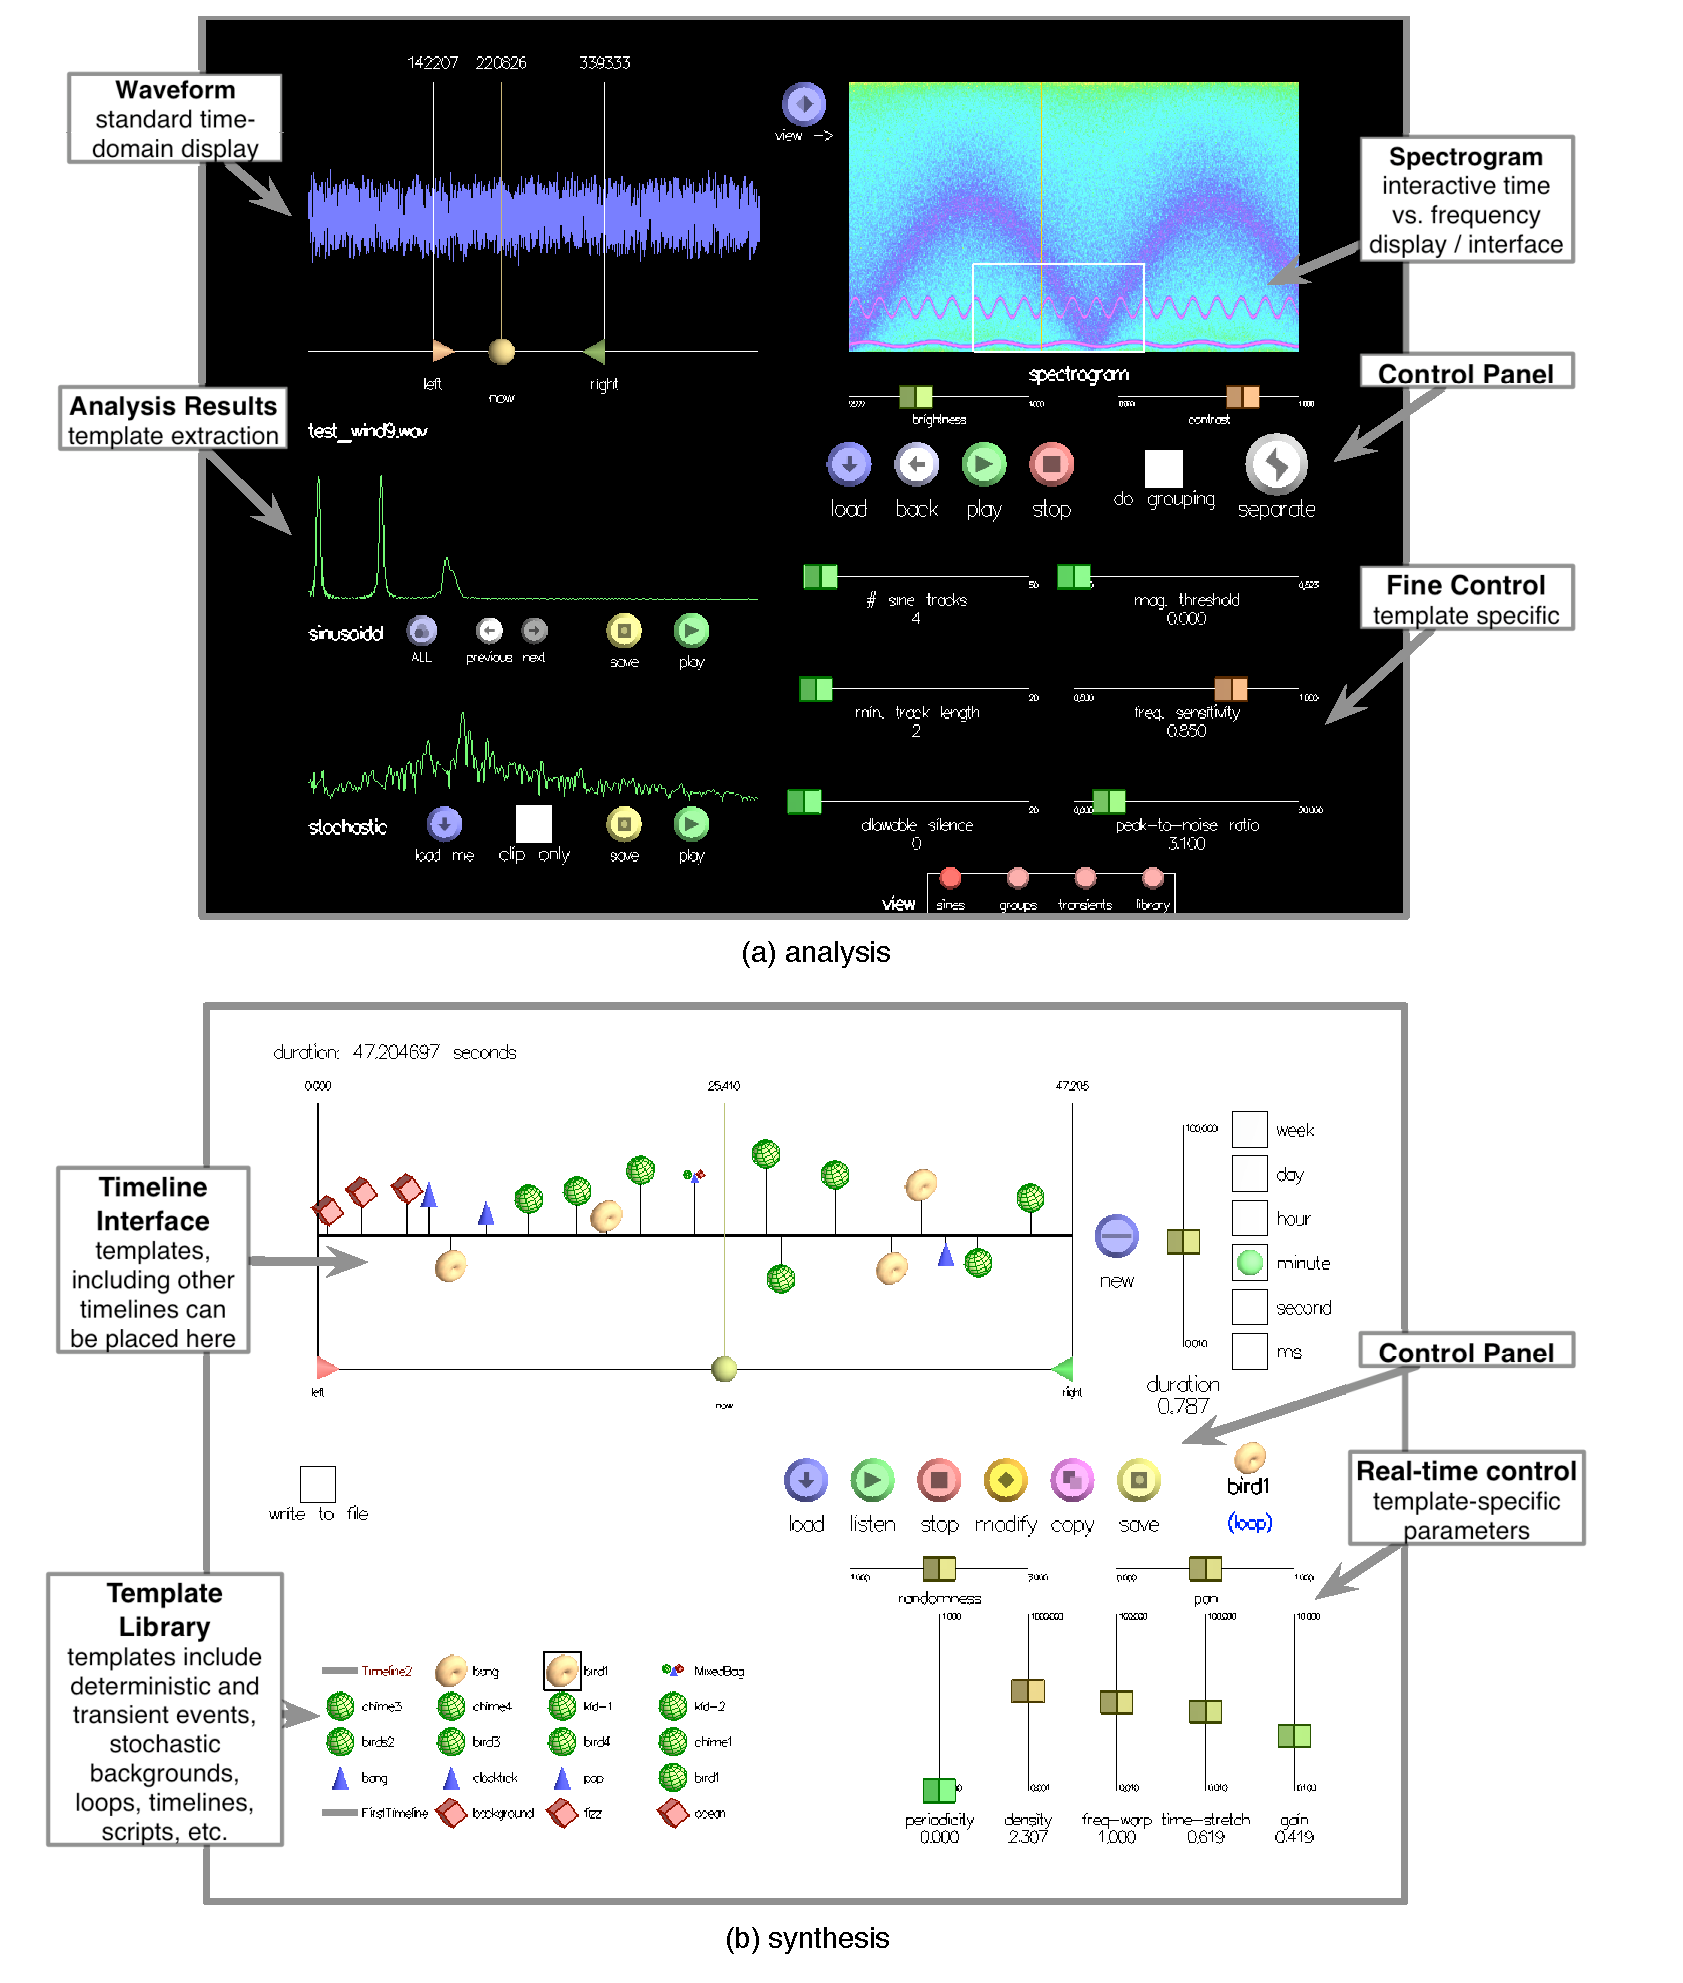
\includegraphics[width=.83\textwidth]{ui2.eps}
%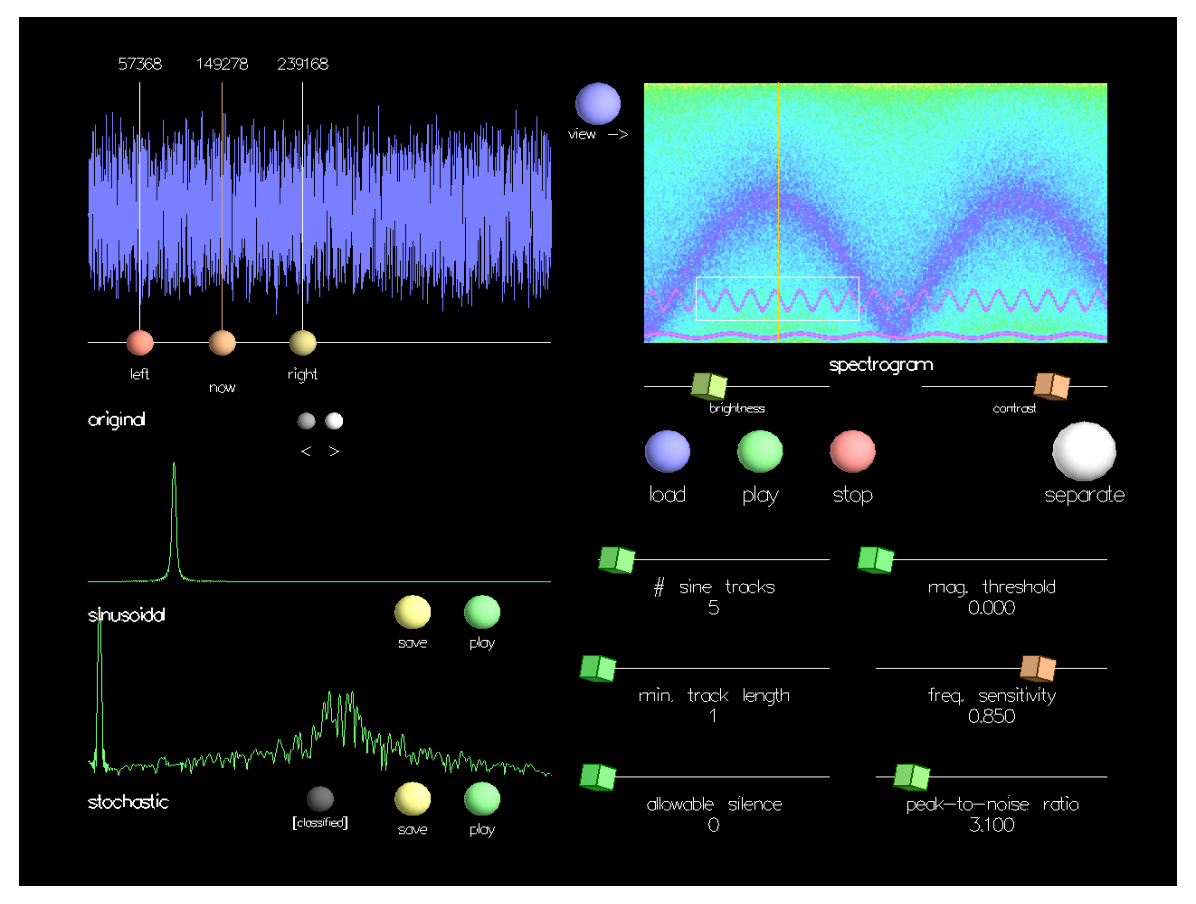
\includegraphics[width=\textwidth]{ui_analysis.eps}
%\subfigure[analysis]{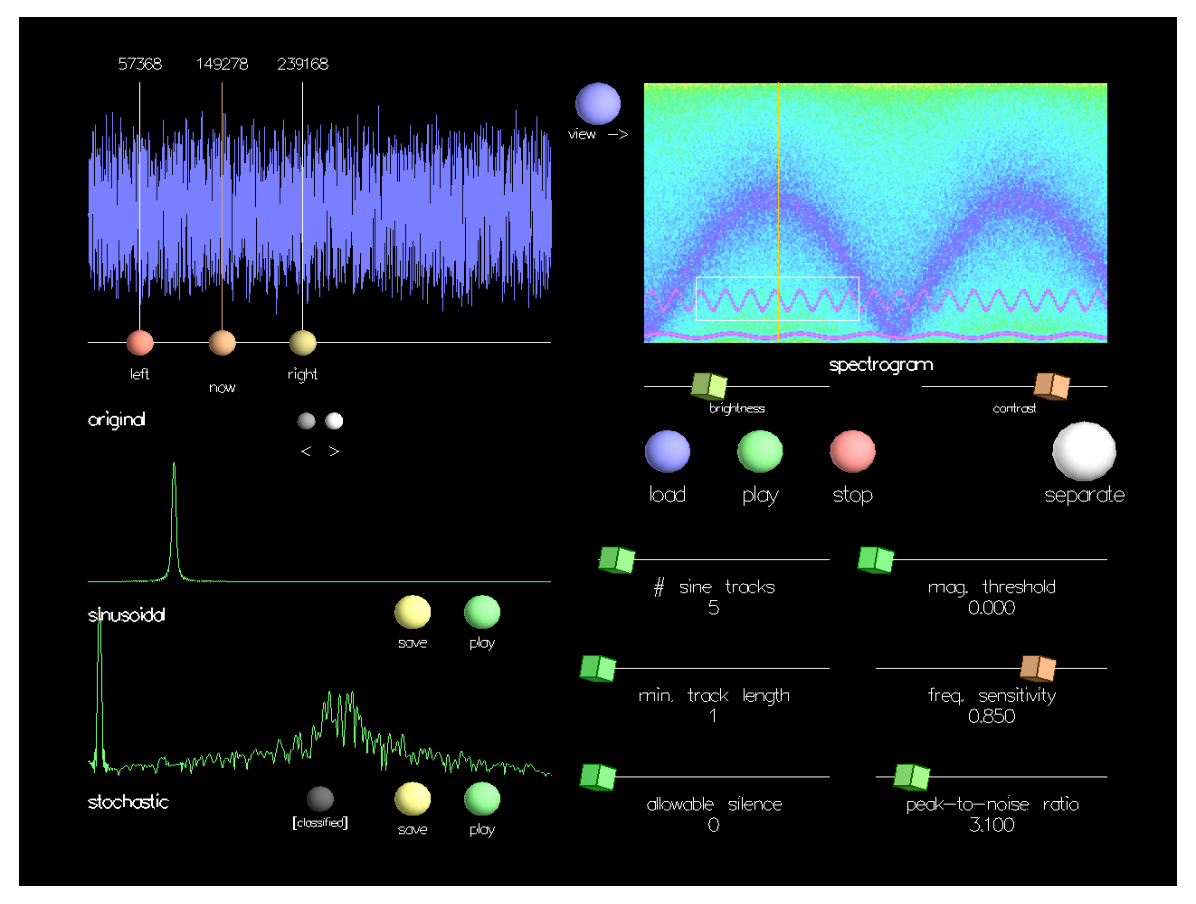
\includegraphics[width=.44\textwidth]{ui_analysis.eps}}
%\subfigure[synthesis]{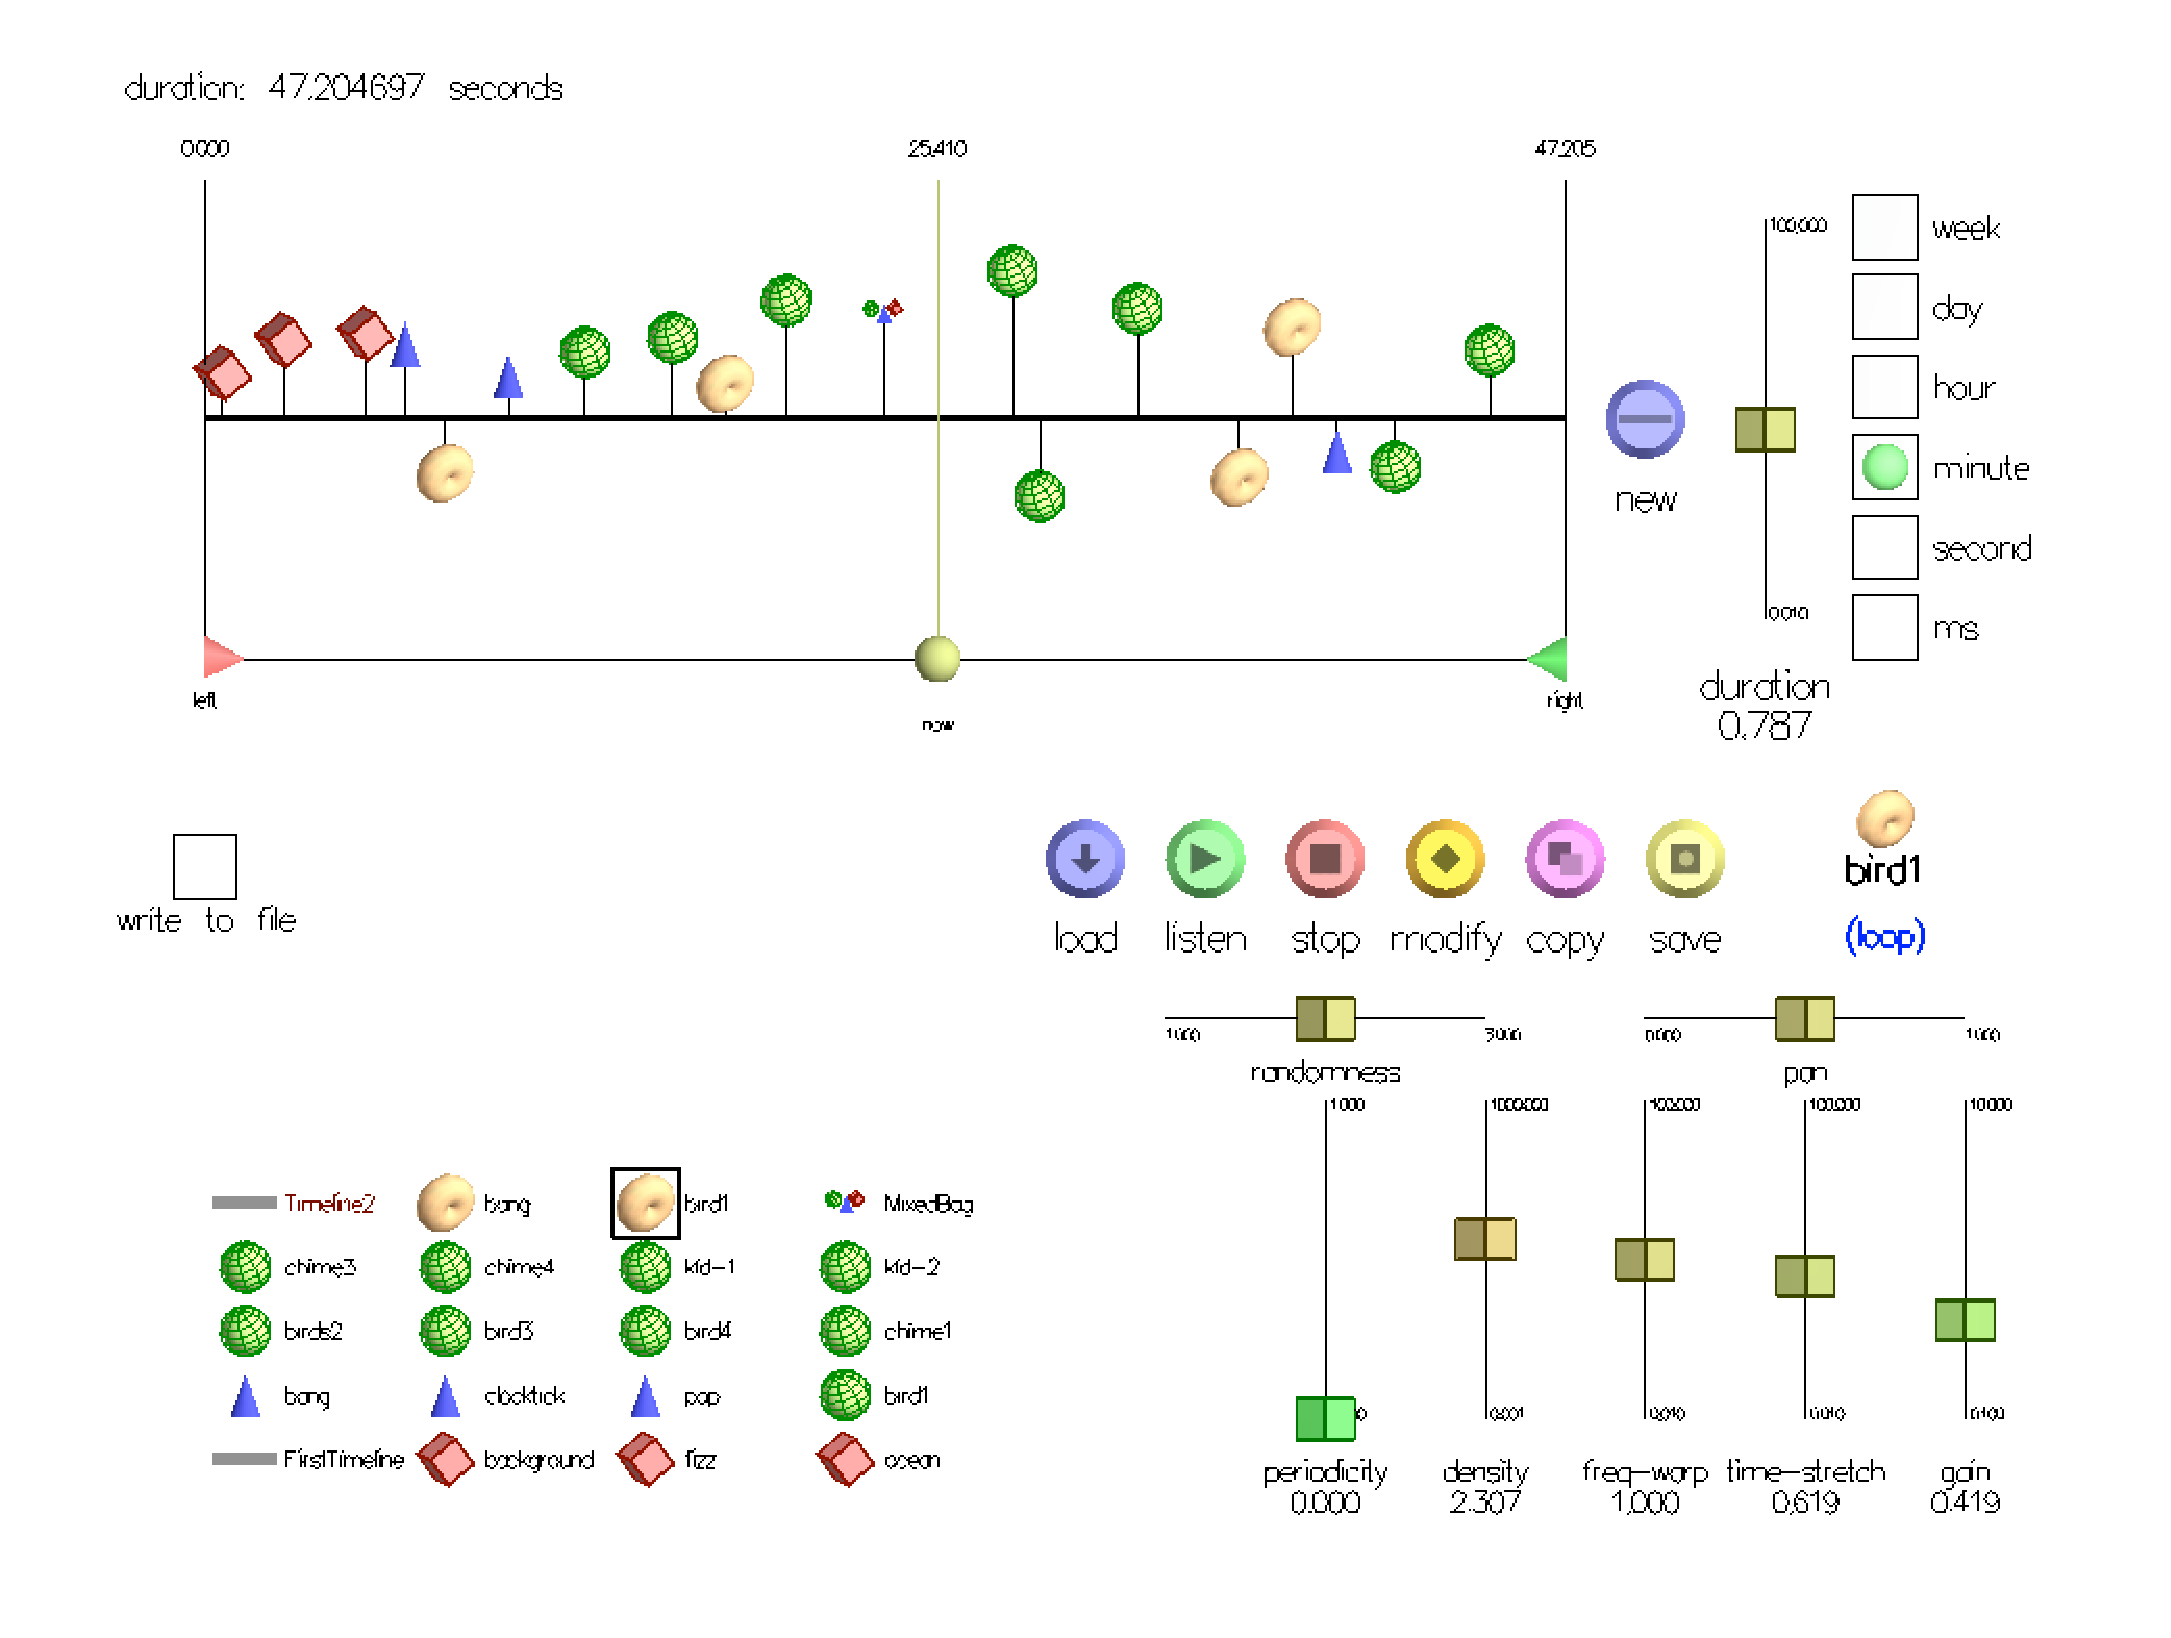
\includegraphics[width=.44\textwidth]{ui_synthesis.eps}}
\caption{Screen shots of user interface. (a) Analysis: Top-left shows time-domain waveform 
while top-right shows spectrogram. Separated spectra are at bottom-left 
and analysis parameters at bottom-right. (b) Synthesis: Top half shows a timeline with 
templates placed on it. Bottom-left shows templates in library; bottom-right shows controls 
for selected loop template.} \clearpage \label{fig:ui}
\end{figure*}



To construct a sound scene from the extracted templates, background and events are combined 
according to the user's preference. Both the level of involvement required and the 
length of the synthesized sound are flexible. 

A sound scene of a specified length can be generated by placing templates 
on a timeline of the desired length. Moreover, the system can generate infinitely long sound 
scenes. The modified wavelet algorithm sythesizes unlimited background texture, while 
previously extracted events can be temporally placed against the background either with fine 
control or in an automated manner as described in Section 5.1.2. 

This framework adapts to many techniques for synthesizing the final sound. A user may 
craft a sound scene by listening to and adjusting the components separately, based on how they 
sound as a group or individually. The combined sound can then be similarly sculpted. On the other 
hand, the synthesis can also be driven from a game or animation algorithm that specifies 
transformations according to parameters drawn from the game or animation itself.

%Minimal involvement entails stating the parameters at a high level and 
%allowing the various components to do their job. More low-level control 
%would involve listening to and adjusting the synthesized components 
%separately, and then doing the same with the combined sound texture. 
%Some hybrid between these two approaches may also be possible.

\section{User Interface}

The user interface (figure \ref{fig:ui}) is separated into two phases: analysis and 
synthesis, both demonstrated in the companion video. 
In the analysis stage, the user can load a sound file and view its waveform, 
frame-by-frame spectrum and spectrogram. These views allow the user to visually 
identify events and perform analysis on appropriate time and frequency regions to
 extract specific events. The waveform is useful for identifying areas of high 
energy in the time domain, which may constitute transient events or sudden loud 
noises. The frame-by-frame spectrum presents a clear view of the sinusoidal 
peaks, and also demonstrates how peak locations change across frames. 
Associated with this view is the absolute magnitude threshold control (Section 4.1), 
which can be visually adjusted and given a spectral tilt according to the characteristics 
of the observed spectrum. Finally, the spectrogram combines time- and frequency-domain 
information in one view. This makes it easy to identify both sinusoidal events 
(near-horizontal lines) and transient events (vertical lines). Time and frequency 
bounds for the analysis can then be specified by adjusting range sliders in the waveform 
and spectrum views or by selecting a rectangle in the spectrogram view. In addition, 
direct control over various other sinusoidal and transient analysis and 
grouping parameters is also available. These parameters have default 
values that have worked well for a range of sounds. 

Once the user has adjusted the analysis parameters or chosen to use the default setting, 
analysis can be started by clicking a button. The extracted events are then played 
separately, along with a frame-by-frame view of their spectrum (for deterministic 
events) or a zoomed in view of their 
waveform (for transient events). The stochastic background can be similarly 
played and viewed, or loaded for further analysis. An 
extracted event or background can optionally be saved as a template for use in 
the synthesis phase. 
The user can then proceed to perform further analysis on the same source sound or 
a different one. 

The synthesis phase of the interface offers a framework for applying 
transformations as well as synthesizing the resulting sounds. Templates 
saved from the analysis stage are available in the synthesis stage for 
listening, transforming, and placing in a sound scene. Templates can be 
of the following types: (1) \emph{deterministic events}, (2) \emph{transient events}, (3) 
\emph{stochastic background}, (4) \emph{loops}, and (5) \emph{timelines}. 
%(1) Deterministic events\\
%(2) Transient events\\
%(3) Stochastic background\\
%(4) Loops\\
%(5) Timelines
The first three are imported directly from the analysis results, and the 
transformations available for these are detailed in Section 5. Loops 
and timelines, briefly described in Section 5.1, help control the temporal 
placement of components in a 
sound scene. Any event can be saved as a loop, with parameters that 
specify how often it repeats and how periodic versus random the 
repetition is. Individual event instances within a loop can also be 
randomly transformed within a controllable range, so that every 
iteration of the loop sounds slightly different. This is useful in 
generating `crowd' sounds, such as a flock of birds constructed from a 
single extracted chirp, or many people from a single voice. 

While loops parametrically repeat a single event, timelines control the 
temporal placement of any number of components. The duration of a timeline 
is specified on creation and can also be changed subsequently. 
Any existing template can be dragged on to the timeline; its location on the 
timeline determines when it is synthesized. 
When the timeline is played, each template on it is synthesized at the appropriate 
time step and played for its duration or until the timeline ends. 
It is also possible to place 
timelines within timelines, thus capturing details of a sound scene at different 
temporal resolutions. Any synthesized sound scene can be written to file while it 
plays, or play forever.  

\section{Results and Contributions}

%Happy Chinese new year

%Using the TAPESTREA framework, we have produced the following examples, shown here as 
%spectrogram plots (and also available in the supplementary audio material).
%, if you can find the supplementary audio material).

%[2-3 large spectogram plots, like in Dubnov et. al ?] Figure \ref{fig:teaser}
%yes but for now ... :S

Examples produced using the TAPESTREA framework include the sound scene shown in Figure 
~\ref{fig:teaser}. This scene is 
composed of four existing sound scenes: (1) a boat-yard, (2) 
a playground, (3) a firecracker whistling and then exploding, and (4) an ocean scene with 
birds. The synthesized sound scene takes place against the ocean background, with foreground 
events consisting of a single bird chirp followed by the train whistle, several fireworks 
exploding, a child screaming, and finally a flock of birds. 
%Are you still there?

Figure ~\ref{fig:traffic} shows another example produced by taking a single 
existing sound scene and transforming it into a different one. 
An original file of length 6 seconds was recorded from a warehouse
environment, with some background noise, a multi-toot horn,
and a door slamming.  The multi-toot horn
was extracted using sinusoidal analysis,
saving multi-toot and single-toot templates.  The
door-slam transient was extracted, leaving
the final stochastic background sound.  A new
scene of length 19 seconds was constructed
using randomized non-looping wavelet
tree re-synthesis for the background.  The
new scene combines multiple and overlapping versions
of frequency and time shifted single horns,
a multi-toot horn, and door slams (some transformed
so greatly that they sound like explosions). 
%The audio for this example is available 
%in the supplemental audio material.
%\dag. 

\begin{figure}[h]
\centering
\includegraphics[width=\columnwidth]{traffic.eps}
\caption{Existing sound scene (top) lengthened and transformed (bottom) with time and frequency 
shifts and continuous background re-synthesis}
\label{fig:traffic}
\end{figure}

Our main contributions comprise of the approach and framework for analysis, transformation, 
and synthesis of sound scenes.  In particular, they are (1) techniques and paradigms for 
automatic and interactive selection and extraction of templates from a sound scene, (2) 
techniques for parametrically transforming components independently of each other, (3) a 
framework for flexible re-synthesis of events and synthesis of novel sound scenes, (4) an 
interface to facilitate each task in the analysis and synthesis pipeline.  Furthermore, we 
have refined several of the core algorithms employed in our system, as follows.

Firstly, we extend the wavelet based background analysis/synthesis algorithm to 
continually resynthesize the background component. In the original algorithm, continual 
re-synthesis is difficult due to the large amount of time taken to learn the highest detail 
levels of the wavelet tree. Stopping the learning at a lower level improves 
the efficiency of the algorithm without significant perceptual cost. The results
%\dag 
in Table 
\ref{tab:treesynth} were obtained by applying the 
original and modified wavelet tree learning on a sound clip of length 18 seconds (sample rate 
11 kHz) to generate 1 minute 58 second sound clips. These show a 4x speedup in 
total running time between the default algorithm (c) and our modified version (b), even 
taking into account the additional expense we incur by consulting a growing number of 
predecessor nodes at each level. The clips synthesized at this additional expense tend to 
sound more stable.

\begin{table}[h]
\begin{center}
\begin{tabular}{|l|c|c|c|}
\hline
  & Learning stop level & Predecessors (k) & Time (sec) \\ \hline
(a) & 9 & fixed & 1.5 \\
(b) & 9 & varying & 1.5 \\
(c) & 15 & fixed & 6 \\
(d) & 15 & varying & 12 \\ \hline
\end{tabular}
\caption{Wavelet tree learning performance results: 
Computations took place at error threshold 25\%. The number of predecessors 
consulted was {\bf fixed} at 5 for all levels, or {\bf varying} as 0.3 times 
the number of nodes in the level. The original sound decomposed into a {\bf 15-level} 
wavelet tree; the modified algorithm stopped learning after {\bf level 9}.} 
\label{tab:treesynth}
\end{center}
\end{table}

Secondly, we refine the sinusoidal extraction process that is a critical task in our sound 
scene analysis. The system provides the option of pre-computing sinusoidal peaks, which
results in performance gains of up to 80\% (typical extractions take on the order of milliseconds to seconds), depending on the analysis parameters used. The 
system also 
implements data structures for grouping sinusoidal tracks and storing these groups as 
objects, which is a first step towards object classification and computational auditory scene analysis ~\cite{Bregman90}. 
%[However, we don't mention these data structures in the paper yet, right?  If not, should 
%we?].  We do.
%The system provides the option of pre-computing sinusoids and potential 
%tracks, and also implements data structures for storing and grouping sinusoidal tracks 
%Results show an average per-extraction performance gain of 0\% [replace with 
%actual results].

Thirdly, we use wavelet tree learning on neighboring areas to fill in the gap left by 
transient removal.  Section 4.2 describes this process.  A clear sonic difference
%\dag 
can be discerned between attenuating the transient segment to the noise floor versus cutting 
out the transient and automatically filling the hole with a stochastic sound clip 
produced by wavelet tree learning. 

In addition, TAPESTREA simplifies the creation of complex sound scenes. Using existing 
tools to create a sound scene can be a tedious process. For example, 
to create a scene with a firework display and a flock of birds over an ocean background, a 
sound designer would need to locate acceptable ``untainted'' versions of the individual 
component sounds as a starting point. These sounds, if found, might not be long 
enough to generate an arbitrary amount of background, forcing the designer to cut, paste, 
reorder and repeat clips, and still risk having perceivable recycling artifacts. Similarly, 
building a flock from one or two birds or a firework display from one or 
two firework sounds would be a multi-step process. The designer would need to manually cut, 
paste, copy, reorder, and transform each clip individually. Having created a scene in this 
way, the designer may need to repeat the entire process just to modify one parameter of 
the scene. 

In contrast, the real-time aspects of our synthesis engine and interface, including 
randomized loops, nested timelines, unlimited and controllable background synthesis, and 
arbitrary randomizable time and frequency transforms, allow fast control over the 
characteristics of the synthesized sound. Moreover, TAPESTREA can: (1) extract sound 
components from complex sounds, (2) synthesize a complete sound scene incorporating 
information from a game, virtual reality system, or multimedia engine, in real-time 
with parametric control, (3) leverage parametric sinusoidal modeling to transform 
deterministic components on a larger scale than other tools, and (4) synthesize unlimited 
non-repeating background via controlled wavelet tree randomization and re-synthesis. 

Our framework is, to our knowledge, the first to classify a sound scene into its 
deterministic, transient, and stochastic components and to provide a comprehensive approach 
for extracting/transforming/resynthesizing the three types of component templates, first
individually, then into cohesive sound scenes.


%A scientific evaluation of the system is difficult, for there are no systematic metrics for 
%testing the perception of sonic reality [need reference here?].  Furthermore, there is 
%nothing like this to compare to: existing sound editors do not do the object identification, 
%group, and separation that ours does.  POTENTIAL EVALUATION: We compared the 
%extraction/synthesis of two segments from different sound scenes using a standard sound 
%editor vs. using our system.  The resulting spectrograms (Figure ??) and the supplementary 
%audio companion (Track ??) highlight the differences between (1) splicing clips, (2) 
%cross-fading clips, and finally (3) using our system to selectively extract foreground and 
%background components, transforming, and rendering them into a conjugate scene.  In this 
%comparison, the continuity of the background and the controllable transformation of 
%foreground objects are two immediate advantages of our system.

%FIX THIS FOR A BETTER FIGURE, BIRDS, KIDS, WHATEVER SHOWS UP BEST IN A 
%SPECTROGRAM.  
%Figure \ref{fig:teaser} describes the effect of sinusoidal 
%separation. Figure 1(a) shows the spectogram of a sound texture made up 
%of two tones (the red horizontal lines) played separately against the 
%background of a typewriter sound. After sinusoidal analysis and 
%re-synthesis, the tones are isolated, as shown in the spectogram in 
%Figure 1(b). 

%Since the typewriter noise 
%(Figure 1(c)) is stochastic, it becomes the background, although the 
%individual typewriter clicks could also be interpreted and generated as 
%stochastic events. Figure 1(d) is our visualization of a synthesized 
%texture based on the sinusoidal separation. The synthesized typewriter 
%background is similar but not identical to the original background in 
%Figure 1(c). The sinusoidal events are made to occur at different time 
%intervals, and last for different amounts of time. Some of them are also 
%pitch-shifted.

%more figures and results go here.  use imagination.

%\subsection{Implementation}
%       - architecture
%\subsection{Sound Examples}
%       - classes of sound\\
%Objectively describe example sounds and results. Have some figures. 

%       - put earlier: waveform at various stages of the pipeline\\
%       - (need a web page)\\
%\subsection{Evaluation}
%We have not yet evaluated our method since we are still completing the 
%implementation. Primary results are promising. When we get to the 
%evaluation stage, we can judge our system based on either the ``actual'' 
%similarity of the synthesized texture to the original, or by their 
%perceptual similarity. The former would require identifying or defining a 
%suitable error metric, while the latter would involve designing and 
%conducting (and participating in) a user study. Since our goal is to 
%generate the sound texture that the user wants to hear, a user study is 
%important.  However, a good error metric would also be useful.
%Evaluate above examples.
%Shirley's idea of having someone construct a new sound texture from existing
%ones and an example to replicate. 
%(THe souhd of slence)

%However, a good error metric would also be useful for 
%judging the psychology soundness of the users.

%However, a technical error metric would also be useful for 
%preliminary testing or for contradicting the results of the user study if 
%necessary. 

%       - error metrics\\
%       - user study\\


\section{Conclusion and Future Work}

We have described a framework for synthesizing unlimited length, perceptually convincing 
sound scenes with separate control over individual foreground events and the background.  
Given an input sound, the system can automatically locate and isolate deterministic 
and transient events, which can then be transformed and placed into new sound scenes 
as individual occurrences or in groups.  Our framework 
also allows users to interactively highlight points of interest in the input 
sound to isolate as 
events.  The background texture is also isolated and saved as a reusable template. This 
separation allows for components to be transformed independently and provides a way to 
combine specific elements from completely different sound scenes.

Unlike existing approaches, our framework separates a given sound into well-defined 
components, which fundamentally allows a greater 
level of control over the variety and quality of the synthesized texture.
We have also demonstrated an interactive paradigm for building new sound scenes, which 
includes iterative refinement of components, interactive previews of transformations, 
grouping, and placement 
in time and space.  Due to the separation, our system is effective in analyzing and 
synthesizing many classes of sounds. %(this is not true at the moment).

While our system has no fundamental restriction on the type of input sound to analyze,
%model,
there are some limitations. When two events have overlapping spectra, it can be hard for the
analysis to distinguish between them. Also, when events have strong deterministic as well as 
stochastic components, these components get separated and may be difficult to regroup. 
%Can regroup with a timeline, but what if you want them in a loop? Can timelines be in loops?
Of course, this can also be viewed as an advantage as it allows components to be 
mixed in different ways. 
%What about events that have strong deterministic and stochastic 
%components?  What about long time-scale events with complex temporal and spectral behavior?
%Example: like a motorcycle? Also, foreground vocals (such as children singing/yelling) or many 
%musical sounds are difficult to capture faithfully.

Future work includes overcoming these limitations by using more sophisticated transient 
detection and deterministic event tracking and grouping methods. We also hope to extend the 
idea of objects to include composite objects containing both deterministic and transient 
components. In addition, we would like to combine machine learning techniques to (1) classify 
events, and (2) allow the system to learn from the user so that performance improves without 
human assistance over time. Although the current defaults work well in general, machine 
learning could be used, for instance, to set  default parameters based on the characteristics 
of the sound being analyzed, for even better automated results. Finally, we would like to 
extend the pre-computing capacities of the system. While preprocessing the sinusoidal peaks 
can provide some speedup in the analysis stage, it may also be possible to pre-match these 
peaks into potential tracks for further performance gain. 

To sum up, our main contributions comprise the approach, system, and interface for 
selective extraction, transformation, and re-synthesis of sound scenes.  While there is 
plenty of scope for future work, TAPESTREA makes it possible to create novel sound scenes 
from existing sounds in a flexible and parametrically controlled manner, providing a new paradigm for both real-time and offline sound production.

%(TODO: future work)  COMBINE MACHINE LEARNING TECHNIQUES TO 1) CLASSIFY EVENTS, 2) LEARN 
%FROM THE USER TO DO %BETTER WITHOUT HUMAN ASSIST OVER TIME. (ALTHOUGH IT WORKS PRETTY GOOD 
%WITH THE DEFAULTS, BLAH BLAH).

\bibliographystyle{acmsiggraph}
\nocite{*}
\bibliography{template}
\end{document}

